\section{Planta}

\begin{frame}{Propostas}

\begin{figure}[htbp]
     \centering
     \begin{subfigure}[t]{0.40\linewidth}
        \centering
        \includegraphics[width=1\linewidth]{tikz/modelo/plantaAntiga.png}
        \caption{Proposta original.}
        \label{fig:simulacoes-1}
     \end{subfigure}
     \begin{subfigure}[t]{0.40\linewidth}
        \centering
        \includegraphics[width=1\linewidth]{tikz/modelo/modelo.png}
        \caption{Proposta nova.}
        \label{fig:simulacoes-2}
     \end{subfigure}
     \caption{Propostas do projeto.}
    \label{fig:simulacoes}
\end{figure}

\end{frame}



\begin{frame}{Nova proposta}

\begin{columns}
    \begin{column}{0.5\textwidth}
        \begin{figure}[htbp]
            \centering
            \resizebox{0.8\textwidth}{!}{


\tikzset{every picture/.style={line width=0.75pt}} %set default line width to 0.75pt        

\begin{tikzpicture}[x=0.75pt,y=0.75pt,yscale=-1,xscale=1]
%uncomment if require: \path (0,682); %set diagram left start at 0, and has height of 682

%Image [id:dp0791029514129229] 
\draw (390,240) node  {\includegraphics[width=315pt,height=300pt]{tikz/modelo/modelo.png}};
%Straight Lines [id:da12694700194316932] 
\draw [color={rgb, 255:red, 189; green, 16; blue, 224 }  ,draw opacity=1 ][line width=3.75]    (220,125) -- (390,125) -- (390,145) -- (310,145) -- (310,220) -- (564,220) ;
\draw [shift={(570,220)}, rotate = 180] [color={rgb, 255:red, 189; green, 16; blue, 224 }  ,draw opacity=1 ][line width=3.75]    (25.14,-7.57) .. controls (15.99,-3.21) and (7.61,-0.69) .. (0,0) .. controls (7.61,0.69) and (15.99,3.21) .. (25.14,7.57)   ;
%Straight Lines [id:da29542059738648274] 
\draw [color={rgb, 255:red, 126; green, 211; blue, 33 }  ,draw opacity=1 ][line width=3.75]    (220,130) -- (385,130) -- (385,140) -- (305,140) -- (305,225) -- (305,399) ;
\draw [shift={(305,405)}, rotate = 270] [color={rgb, 255:red, 126; green, 211; blue, 33 }  ,draw opacity=1 ][line width=3.75]    (25.14,-7.57) .. controls (15.99,-3.21) and (7.61,-0.69) .. (0,0) .. controls (7.61,0.69) and (15.99,3.21) .. (25.14,7.57)   ;

% Text Node
\draw (225,85) node  [font=\large] [align=left] {\begin{minipage}[lt]{41.14pt}\setlength\topsep{0pt}
\begin{center}
SF
\end{center}

\end{minipage}};
% Text Node
\draw (305,85) node  [font=\large] [align=left] {\begin{minipage}[lt]{41.14pt}\setlength\topsep{0pt}
\begin{center}
RB
\end{center}

\end{minipage}};
% Text Node
\draw (455,130) node  [font=\large] [align=left] {\begin{minipage}[lt]{41.14pt}\setlength\topsep{0pt}
\begin{center}
PM1
\end{center}

\end{minipage}};
% Text Node
\draw (235,250) node  [font=\large] [align=left] {\begin{minipage}[lt]{41.14pt}\setlength\topsep{0pt}
\begin{center}
DS
\end{center}

\end{minipage}};
% Text Node
\draw (235,410) node  [font=\large] [align=left] {\begin{minipage}[lt]{41.14pt}\setlength\topsep{0pt}
\begin{center}
XS1
\end{center}

\end{minipage}};
% Text Node
\draw (550,270) node  [font=\large] [align=left] {\begin{minipage}[lt]{41.14pt}\setlength\topsep{0pt}
\begin{center}
XS2
\end{center}

\end{minipage}};
% Text Node
\draw (390,320) node  [font=\large] [align=left] {\begin{minipage}[lt]{41.14pt}\setlength\topsep{0pt}
\begin{center}
PM2
\end{center}

\end{minipage}};


\end{tikzpicture}}
            \caption{Planta para a máquina de \textit{milkshake}.}
            \label{fig:sistema}
        \end{figure}
    \end{column}
    \begin{column}{0.5\textwidth}
        \begin{figure}[htbp]
            \centering
            \begin{minipage}{\textwidth}
                \centering
                \resizebox{0.2\textwidth}{!}
                {


\tikzset{every picture/.style={line width=0.75pt}} %set default line width to 0.75pt        


\begin{tikzpicture}[x=0.75pt,y=0.75pt,yscale=-1,xscale=1]
%uncomment if require: \path (0,300); %set diagram left start at 0, and has height of 300

%Curve Lines [id:da33623388382234665] 
\draw [draw opacity=0][fill={rgb, 255:red, 255; green, 255; blue, 255 }  ,fill opacity=1 ][line width=0.75] [line join = round][line cap = round]   (215.8,98.12) .. controls (218.97,99.2) and (223.27,104.03) .. (225.3,101.37) .. controls (233.8,85.17) and (240.3,71.17) .. (245.55,59.12) .. controls (246.45,55.63) and (240.48,48.25) .. (238.3,51.12) .. controls (231.05,62.67) and (223.63,82.12) .. (216.3,97.62) ;
%Curve Lines [id:da6517219999182808] 
\draw [draw opacity=0][fill={rgb, 255:red, 255; green, 255; blue, 255 }  ,fill opacity=1 ][line width=0.75] [line join = round][line cap = round]   (238.05,50.92) .. controls (240.3,47.42) and (242.78,43.66) .. (246.3,44.17) .. controls (250.56,44.78) and (253.17,49.68) .. (255.3,53.42) .. controls (260.05,64.42) and (263.3,71.17) .. (270.5,85.92) .. controls (271.08,88.99) and (264.5,94.12) .. (262.55,91.67) .. controls (257.55,81.17) and (253.55,70.92) .. (247.05,57.42) .. controls (248.05,54.67) and (245.56,60.93) .. (244.3,60.42) .. controls (240.76,58.98) and (235.84,54.58) .. (237.55,51.17) ;
%Curve Lines [id:da33392627803622843] 
\draw [draw opacity=0][fill={rgb, 255:red, 208; green, 2; blue, 27 }  ,fill opacity=1 ][line width=0.75] [line join = round][line cap = round]   (268.05,81.17) .. controls (268.3,84.17) and (267.16,87.64) .. (268.8,90.17) .. controls (268.58,91.42) and (272.58,88.17) .. (268.8,82.17) ;
%Curve Lines [id:da05524754410677479] 
\draw [draw opacity=0][fill={rgb, 255:red, 208; green, 2; blue, 27 }  ,fill opacity=1 ][line width=0.75] [line join = round][line cap = round]   (259.05,63.42) .. controls (258.72,69.83) and (259.8,76.92) .. (258.8,81.67) .. controls (259.03,83.74) and (261.29,89.69) .. (261.8,87.67) .. controls (263.05,71.42) and (264.52,72.32) .. (260.05,64.67) ;
%Curve Lines [id:da10288432289609939] 
\draw [draw opacity=0][fill={rgb, 255:red, 208; green, 2; blue, 27 }  ,fill opacity=1 ][line width=0.75] [line join = round][line cap = round]   (252.3,47.92) .. controls (251.97,54.33) and (252.08,60.5) .. (252.05,66.17) .. controls (252.28,68.24) and (254.54,74.19) .. (255.05,72.17) .. controls (256.3,55.92) and (256.58,55.75) .. (253.3,49.17) ;
%Curve Lines [id:da48052459184272034] 
\draw [draw opacity=0][fill={rgb, 255:red, 208; green, 2; blue, 27 }  ,fill opacity=1 ][line width=0.75] [line join = round][line cap = round]   (221.25,85.67) .. controls (224.21,82.88) and (241.33,71.42) .. (235.5,80.67) .. controls (234.33,83.17) and (233.79,85.72) .. (231.75,87.17) .. controls (228,87.33) and (219.5,95.83) .. (215,99.33) .. controls (215.5,96.83) and (220.33,87.5) .. (222.25,84.17) ;
%Curve Lines [id:da5565878074443247] 
\draw [draw opacity=0][fill={rgb, 255:red, 208; green, 2; blue, 27 }  ,fill opacity=1 ][line width=0.75] [line join = round][line cap = round]   (237.8,53.17) .. controls (242.05,49.83) and (244.3,46.33) .. (251.3,45.92) .. controls (251.8,46.33) and (247.55,43.83) .. (246.3,44.17) .. controls (240.55,46.08) and (239.3,50.33) .. (238.55,52.42) ;
%Curve Lines [id:da38187296164180884] 
\draw [draw opacity=0][fill={rgb, 255:red, 208; green, 2; blue, 27 }  ,fill opacity=1 ][line width=0.75] [line join = round][line cap = round]   (232.8,62.42) .. controls (235.76,59.63) and (242.05,54.58) .. (247.05,57.42) .. controls (245.55,57.33) and (245.34,62.47) .. (243.3,63.92) .. controls (239.55,64.08) and (231.05,72.58) .. (226.55,76.08) .. controls (227.05,73.58) and (231.88,64.25) .. (233.8,60.92) ;
%Shape: Ellipse [id:dp40094882673661036] 
\draw  [draw opacity=0][line width=2.25]  (150.84,195.84) .. controls (152.87,183.77) and (177.58,177.86) .. (206.03,182.64) .. controls (234.48,187.43) and (255.9,201.08) .. (253.87,213.15) .. controls (251.84,225.22) and (227.14,231.12) .. (198.69,226.34) .. controls (170.24,221.56) and (148.82,207.9) .. (150.84,195.84) -- cycle ;
%Straight Lines [id:da8992804145996609] 
\draw [color={rgb, 255:red, 74; green, 74; blue, 74 }  ,draw opacity=1 ][fill={rgb, 255:red, 155; green, 155; blue, 155 }  ,fill opacity=1 ]   (238.5,49.67) -- (215.5,98.42) ;
%Straight Lines [id:da1621651244646496] 
\draw [color={rgb, 255:red, 74; green, 74; blue, 74 }  ,draw opacity=1 ]   (245.5,59.67) -- (225.5,101.67) ;
%Shape: Arc [id:dp8497438534326236] 
\draw  [draw opacity=0][fill={rgb, 255:red, 252; green, 52; blue, 74 }  ,fill opacity=1 ][line width=2.25]  (237.99,121.53) .. controls (235.96,133.6) and (212.65,139.74) .. (185.92,135.25) .. controls (159.19,130.76) and (139.17,117.33) .. (141.2,105.27) .. controls (143.23,93.2) and (166.54,87.06) .. (193.27,91.55) .. controls (219.99,96.04) and (240.02,109.47) .. (237.99,121.53) -- (189.59,113.4) -- cycle ; \draw  [draw opacity=0][line width=2.25]  (237.99,121.53) .. controls (235.96,133.6) and (212.65,139.74) .. (185.92,135.25) .. controls (159.19,130.76) and (139.17,117.33) .. (141.2,105.27) .. controls (143.23,93.2) and (166.54,87.06) .. (193.27,91.55) .. controls (219.99,96.04) and (240.02,109.47) .. (237.99,121.53) -- cycle ;  
%Curve Lines [id:da6745169594181273] 
\draw [draw opacity=0][fill={rgb, 255:red, 201; green, 195; blue, 195 }  ,fill opacity=0.66 ][line width=0.75] [line join = round][line cap = round]   (141.2,105.27) .. controls (141.2,97.28) and (140.21,80.26) .. (145.2,75.27) .. controls (148.96,71.51) and (157.13,71.28) .. (163.2,70.27) .. controls (189.71,65.85) and (220.53,70.6) .. (235.2,85.27) .. controls (238.08,88.15) and (244.66,90.38) .. (245.2,95.27) .. controls (246.45,106.56) and (240.2,111.49) .. (240.2,121.27) .. controls (240.2,122.47) and (239.05,119.12) .. (238.2,118.27) .. controls (236.27,116.33) and (236.04,111.11) .. (234.2,109.27) .. controls (230.27,105.34) and (213.56,95.86) .. (208.2,95.27) .. controls (191.63,93.43) and (186.78,90.4) .. (164.2,91.27) .. controls (159.82,91.44) and (153.98,93.67) .. (149.2,95.27) .. controls (145.95,96.35) and (144.7,103.27) .. (141.2,103.27) ;
%Shape: Trapezoid [id:dp9836029479786901] 
\draw  [draw opacity=0][fill={rgb, 255:red, 252; green, 52; blue, 74 }  ,fill opacity=1 ] (238.5,125.93) -- (205.79,237.18) -- (139.82,223.54) -- (142.27,106.04) -- cycle ;
%Shape: Arc [id:dp10237578178410933] 
\draw  [draw opacity=0][line width=2.25]  (142.83,83.67) .. controls (142.83,83.67) and (142.83,83.67) .. (142.83,83.67) .. controls (144.85,71.6) and (169.56,65.69) .. (198.01,70.48) .. controls (226.46,75.26) and (247.88,88.91) .. (245.85,100.98) -- (194.34,92.32) -- cycle ; \draw  [line width=2.25]  (142.83,83.67) .. controls (142.83,83.67) and (142.83,83.67) .. (142.83,83.67) .. controls (144.85,71.6) and (169.56,65.69) .. (198.01,70.48) .. controls (226.46,75.26) and (247.88,88.91) .. (245.85,100.98) ;  
%Shape: Ellipse [id:dp926473623529513] 
\draw  [line width=2.25]  (139.48,224.75) .. controls (140.18,220.59) and (155.52,219.7) .. (173.76,222.76) .. controls (191.99,225.82) and (206.21,231.68) .. (205.51,235.85) .. controls (204.81,240.01) and (189.46,240.9) .. (171.22,237.84) .. controls (152.99,234.77) and (138.78,228.91) .. (139.48,224.75) -- cycle ;
%Shape: Ellipse [id:dp042692779544714066] 
\draw  [fill={rgb, 255:red, 252; green, 52; blue, 74 }  ,fill opacity=1 ][line width=2.25]  (139.48,224.75) .. controls (140.18,220.59) and (155.52,219.7) .. (173.76,222.76) .. controls (191.99,225.82) and (206.21,231.68) .. (205.51,235.85) .. controls (204.81,240.01) and (189.46,240.9) .. (171.22,237.84) .. controls (152.99,234.77) and (138.78,228.91) .. (139.48,224.75) -- cycle ;
%Straight Lines [id:da7389947599407996] 
\draw [line width=2.25]    (139.48,224.75) -- (142.83,83.67) ;
%Straight Lines [id:da9728249678309886] 
\draw [line width=2.25]    (245.85,100.98) -- (205.51,235.85) ;
%Shape: Arc [id:dp3932843359864808] 
\draw  [draw opacity=0][fill={rgb, 255:red, 252; green, 52; blue, 74 }  ,fill opacity=1 ][line width=2.25]  (142.27,106.04) .. controls (144.3,93.97) and (167.61,87.83) .. (194.34,92.32) .. controls (221.07,96.82) and (241.09,110.24) .. (239.06,122.31) -- (190.67,114.17) -- cycle ; \draw  [line width=2.25]  (142.27,106.04) .. controls (144.3,93.97) and (167.61,87.83) .. (194.34,92.32) .. controls (221.07,96.82) and (241.09,110.24) .. (239.06,122.31) ;  
%Straight Lines [id:da8573053213137072] 
\draw [color={rgb, 255:red, 74; green, 74; blue, 74 }  ,draw opacity=1 ]   (248.75,60.17) -- (262.25,91.17) ;
%Straight Lines [id:da7298578047225213] 
\draw [color={rgb, 255:red, 74; green, 74; blue, 74 }  ,draw opacity=1 ]   (253.5,49.92) -- (270.5,85.92) ;
%Shape: Arc [id:dp15110507933656647] 
\draw  [draw opacity=0] (238.21,50.63) .. controls (240.06,46.83) and (242.88,44.41) .. (246.04,44.41) .. controls (248.99,44.41) and (251.65,46.53) .. (253.5,49.92) -- (246.04,61.41) -- cycle ; \draw  [color={rgb, 255:red, 74; green, 74; blue, 74 }  ,draw opacity=1 ] (238.21,50.63) .. controls (240.06,46.83) and (242.88,44.41) .. (246.04,44.41) .. controls (248.99,44.41) and (251.65,46.53) .. (253.5,49.92) ;  
%Shape: Arc [id:dp2274995624393623] 
\draw  [draw opacity=0] (245.1,60.59) .. controls (245.51,58.98) and (246.22,57.92) .. (247.03,57.92) .. controls (247.8,57.92) and (248.48,58.89) .. (248.89,60.38) -- (247.03,63.67) -- cycle ; \draw  [color={rgb, 255:red, 74; green, 74; blue, 74 }  ,draw opacity=1 ] (245.1,60.59) .. controls (245.51,58.98) and (246.22,57.92) .. (247.03,57.92) .. controls (247.8,57.92) and (248.48,58.89) .. (248.89,60.38) ;  
%Shape: Arc [id:dp4687377714663463] 
\draw  [draw opacity=0] (269.81,84.27) .. controls (269.81,84.27) and (269.81,84.27) .. (269.81,84.27) .. controls (271.3,86.15) and (270.71,89.09) .. (268.5,90.84) .. controls (266.29,92.59) and (263.3,92.49) .. (261.81,90.61) -- (265.81,87.44) -- cycle ; \draw  [color={rgb, 255:red, 74; green, 74; blue, 74 }  ,draw opacity=1 ] (269.81,84.27) .. controls (269.81,84.27) and (269.81,84.27) .. (269.81,84.27) .. controls (271.3,86.15) and (270.71,89.09) .. (268.5,90.84) .. controls (266.29,92.59) and (263.3,92.49) .. (261.81,90.61) ;  




\end{tikzpicture}}
                \subcaption{\textit{Milkshake} \textbf{sem} cobertura.}\label{fig:milk_00}
            \end{minipage}
            \begin{minipage}{\textwidth}
                \centering
                \resizebox{0.2\textwidth}{!}
                {


\tikzset{every picture/.style={line width=0.75pt}} %set default line width to 0.75pt        

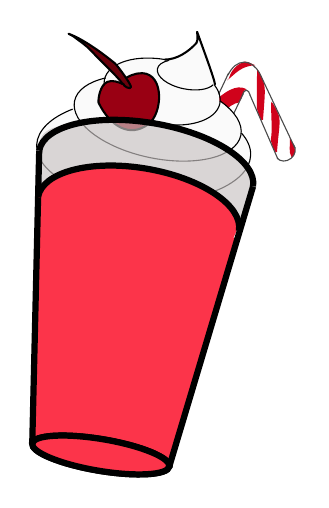
\begin{tikzpicture}[x=0.75pt,y=0.75pt,yscale=-1,xscale=1]
%uncomment if require: \path (0,800); %set diagram left start at 0, and has height of 800

%Curve Lines [id:da7965757231260868] 
\draw [draw opacity=0][fill={rgb, 255:red, 255; green, 255; blue, 255 }  ,fill opacity=1 ][line width=0.75] [line join = round][line cap = round]   (202.6,412.72) .. controls (205.77,413.8) and (210.07,418.63) .. (212.1,415.97) .. controls (220.6,399.77) and (227.1,385.77) .. (232.35,373.72) .. controls (233.25,370.23) and (227.28,362.85) .. (225.1,365.72) .. controls (217.85,377.27) and (210.43,396.72) .. (203.1,412.22) ;
%Curve Lines [id:da08719065296182538] 
\draw [draw opacity=0][fill={rgb, 255:red, 255; green, 255; blue, 255 }  ,fill opacity=1 ][line width=0.75] [line join = round][line cap = round]   (224.85,365.52) .. controls (227.1,362.02) and (229.58,358.26) .. (233.1,358.77) .. controls (237.36,359.38) and (239.97,364.28) .. (242.1,368.02) .. controls (246.85,379.02) and (250.1,385.77) .. (257.3,400.52) .. controls (257.88,403.59) and (251.3,408.72) .. (249.35,406.27) .. controls (244.35,395.77) and (240.35,385.52) .. (233.85,372.02) .. controls (234.85,369.27) and (232.36,375.53) .. (231.1,375.02) .. controls (227.56,373.58) and (222.64,369.18) .. (224.35,365.77) ;
%Curve Lines [id:da4690184172645433] 
\draw [draw opacity=0][fill={rgb, 255:red, 208; green, 2; blue, 27 }  ,fill opacity=1 ][line width=0.75] [line join = round][line cap = round]   (254.85,395.77) .. controls (255.1,398.77) and (253.96,402.24) .. (255.6,404.77) .. controls (255.38,406.02) and (259.38,402.77) .. (255.6,396.77) ;
%Curve Lines [id:da4519840618426807] 
\draw [draw opacity=0][fill={rgb, 255:red, 208; green, 2; blue, 27 }  ,fill opacity=1 ][line width=0.75] [line join = round][line cap = round]   (245.85,378.02) .. controls (245.52,384.43) and (246.6,391.52) .. (245.6,396.27) .. controls (245.83,398.34) and (248.09,404.29) .. (248.6,402.27) .. controls (249.85,386.02) and (251.32,386.92) .. (246.85,379.27) ;
%Curve Lines [id:da6363354517421407] 
\draw [draw opacity=0][fill={rgb, 255:red, 208; green, 2; blue, 27 }  ,fill opacity=1 ][line width=0.75] [line join = round][line cap = round]   (239.1,362.52) .. controls (238.77,368.93) and (238.88,375.1) .. (238.85,380.77) .. controls (239.08,382.84) and (241.34,388.79) .. (241.85,386.77) .. controls (243.1,370.52) and (243.38,370.35) .. (240.1,363.77) ;
%Curve Lines [id:da835096719025997] 
\draw [draw opacity=0][fill={rgb, 255:red, 208; green, 2; blue, 27 }  ,fill opacity=1 ][line width=0.75] [line join = round][line cap = round]   (208.05,400.27) .. controls (211.01,397.48) and (228.13,386.02) .. (222.3,395.27) .. controls (221.13,397.77) and (220.59,400.32) .. (218.55,401.77) .. controls (214.8,401.93) and (206.3,410.43) .. (201.8,413.93) .. controls (202.3,411.43) and (207.13,402.1) .. (209.05,398.77) ;
%Curve Lines [id:da3369981206119428] 
\draw [draw opacity=0][fill={rgb, 255:red, 208; green, 2; blue, 27 }  ,fill opacity=1 ][line width=0.75] [line join = round][line cap = round]   (224.6,367.77) .. controls (228.85,364.43) and (231.1,360.93) .. (238.1,360.52) .. controls (238.6,360.93) and (234.35,358.43) .. (233.1,358.77) .. controls (227.35,360.68) and (226.1,364.93) .. (225.35,367.02) ;
%Curve Lines [id:da8535933909156281] 
\draw [draw opacity=0][fill={rgb, 255:red, 208; green, 2; blue, 27 }  ,fill opacity=1 ][line width=0.75] [line join = round][line cap = round]   (219.6,377.02) .. controls (222.56,374.23) and (228.85,369.18) .. (233.85,372.02) .. controls (232.35,371.93) and (232.14,377.07) .. (230.1,378.52) .. controls (226.35,378.68) and (217.85,387.18) .. (213.35,390.68) .. controls (213.85,388.18) and (218.68,378.85) .. (220.6,375.52) ;
%Straight Lines [id:da36367926832969744] 
\draw [color={rgb, 255:red, 74; green, 74; blue, 74 }  ,draw opacity=1 ][fill={rgb, 255:red, 155; green, 155; blue, 155 }  ,fill opacity=1 ]   (225.3,364.27) -- (202.3,413.02) ;
%Straight Lines [id:da5239378222022764] 
\draw [color={rgb, 255:red, 74; green, 74; blue, 74 }  ,draw opacity=1 ]   (232.3,374.27) -- (212.3,416.27) ;
%Straight Lines [id:da06920061006817613] 
\draw [color={rgb, 255:red, 74; green, 74; blue, 74 }  ,draw opacity=1 ]   (235.55,374.77) -- (249.05,405.77) ;
%Straight Lines [id:da22092088270054688] 
\draw [color={rgb, 255:red, 74; green, 74; blue, 74 }  ,draw opacity=1 ]   (240.3,364.52) -- (257.3,400.52) ;
%Shape: Arc [id:dp12934255979399922] 
\draw  [draw opacity=0] (225.01,365.23) .. controls (226.86,361.43) and (229.68,359.01) .. (232.84,359.01) .. controls (235.79,359.01) and (238.45,361.13) .. (240.3,364.52) -- (232.84,376.01) -- cycle ; \draw  [color={rgb, 255:red, 74; green, 74; blue, 74 }  ,draw opacity=1 ] (225.01,365.23) .. controls (226.86,361.43) and (229.68,359.01) .. (232.84,359.01) .. controls (235.79,359.01) and (238.45,361.13) .. (240.3,364.52) ;  
%Shape: Arc [id:dp07342029146364548] 
\draw  [draw opacity=0] (231.9,375.19) .. controls (232.31,373.58) and (233.02,372.52) .. (233.83,372.52) .. controls (234.6,372.52) and (235.28,373.49) .. (235.69,374.98) -- (233.83,378.27) -- cycle ; \draw  [color={rgb, 255:red, 74; green, 74; blue, 74 }  ,draw opacity=1 ] (231.9,375.19) .. controls (232.31,373.58) and (233.02,372.52) .. (233.83,372.52) .. controls (234.6,372.52) and (235.28,373.49) .. (235.69,374.98) ;  
%Shape: Arc [id:dp8358607171937402] 
\draw  [draw opacity=0] (256.61,398.87) .. controls (256.61,398.87) and (256.61,398.87) .. (256.61,398.87) .. controls (258.1,400.75) and (257.51,403.69) .. (255.3,405.44) .. controls (253.09,407.19) and (250.1,407.09) .. (248.61,405.21) -- (252.61,402.04) -- cycle ; \draw  [color={rgb, 255:red, 74; green, 74; blue, 74 }  ,draw opacity=1 ] (256.61,398.87) .. controls (256.61,398.87) and (256.61,398.87) .. (256.61,398.87) .. controls (258.1,400.75) and (257.51,403.69) .. (255.3,405.44) .. controls (253.09,407.19) and (250.1,407.09) .. (248.61,405.21) ;  

%Shape: Ellipse [id:dp8665421514125364] 
\draw  [draw opacity=0][fill={rgb, 255:red, 250; green, 250; blue, 250 }  ,fill opacity=1 ] (132.41,398.86) .. controls (133.08,385.27) and (156.71,375.39) .. (185.18,376.81) .. controls (213.65,378.23) and (236.18,390.4) .. (235.5,404) .. controls (234.82,417.59) and (211.19,427.47) .. (182.73,426.05) .. controls (154.26,424.63) and (131.73,412.46) .. (132.41,398.86) -- cycle ;
%Shape: Ellipse [id:dp1329424670534627] 
\draw  [draw opacity=0][fill={rgb, 255:red, 250; green, 250; blue, 250 }  ,fill opacity=1 ] (150.67,377.74) .. controls (152.83,367.26) and (172.52,362.48) .. (194.64,367.06) .. controls (216.76,371.63) and (232.93,383.83) .. (230.77,394.31) .. controls (228.6,404.78) and (208.91,409.57) .. (186.79,404.99) .. controls (164.67,400.41) and (148.5,388.21) .. (150.67,377.74) -- cycle ;
%Shape: Ellipse [id:dp7435760803169824] 
\draw  [draw opacity=0][fill={rgb, 255:red, 250; green, 250; blue, 250 }  ,fill opacity=1 ] (165.07,367.44) .. controls (166.79,359.12) and (180.64,354.94) .. (195.99,358.12) .. controls (211.35,361.3) and (222.4,370.62) .. (220.68,378.95) .. controls (218.96,387.28) and (205.11,391.45) .. (189.76,388.27) .. controls (174.4,385.1) and (163.35,375.77) .. (165.07,367.44) -- cycle ;
%Curve Lines [id:da5244842889211496] 
\draw [draw opacity=0][fill={rgb, 255:red, 250; green, 250; blue, 250 }  ,fill opacity=1 ][line width=0.75] [line join = round][line cap = round]   (194.2,357.8) .. controls (199.93,357.8) and (205.56,354.04) .. (209.4,349.8) .. controls (210.57,348.51) and (209.3,342.93) .. (209.8,344.6) .. controls (210.58,347.19) and (219.06,369.51) .. (218.2,369.8) ;

%Shape: Arc [id:dp7258176709737072] 
\draw  [draw opacity=0] (231.49,393.23) .. controls (234.49,396.58) and (236.09,400.23) .. (235.9,404) .. controls (235.22,417.59) and (211.59,427.47) .. (183.13,426.05) .. controls (154.66,424.63) and (132.13,412.46) .. (132.81,398.86) .. controls (133.16,391.75) and (139.8,385.65) .. (150.14,381.66) -- (184.35,401.43) -- cycle ; \draw   (231.49,393.23) .. controls (234.49,396.58) and (236.09,400.23) .. (235.9,404) .. controls (235.22,417.59) and (211.59,427.47) .. (183.13,426.05) .. controls (154.66,424.63) and (132.13,412.46) .. (132.81,398.86) .. controls (133.16,391.75) and (139.8,385.65) .. (150.14,381.66) ;  
%Shape: Arc [id:dp32184203472359685] 
\draw  [draw opacity=0] (221.15,377.69) .. controls (228.36,382.8) and (232.31,388.79) .. (231.17,394.31) .. controls (229,404.78) and (209.31,409.57) .. (187.19,404.99) .. controls (165.07,400.41) and (148.9,388.21) .. (151.07,377.74) .. controls (152.17,372.39) and (157.84,368.53) .. (166.06,366.64) -- (191.12,386.02) -- cycle ; \draw   (221.15,377.69) .. controls (228.36,382.8) and (232.31,388.79) .. (231.17,394.31) .. controls (229,404.78) and (209.31,409.57) .. (187.19,404.99) .. controls (165.07,400.41) and (148.9,388.21) .. (151.07,377.74) .. controls (152.17,372.39) and (157.84,368.53) .. (166.06,366.64) ;  
%Shape: Arc [id:dp9369100352963733] 
\draw  [draw opacity=0] (218.54,370.12) .. controls (220.71,372.98) and (221.68,376.03) .. (221.08,378.95) .. controls (219.36,387.28) and (205.51,391.45) .. (190.16,388.27) .. controls (174.8,385.1) and (163.75,375.77) .. (165.47,367.44) .. controls (167.19,359.12) and (181.04,354.94) .. (196.39,358.12) .. controls (196.47,358.14) and (196.54,358.15) .. (196.61,358.17) -- (193.28,373.2) -- cycle ; \draw   (218.54,370.12) .. controls (220.71,372.98) and (221.68,376.03) .. (221.08,378.95) .. controls (219.36,387.28) and (205.51,391.45) .. (190.16,388.27) .. controls (174.8,385.1) and (163.75,375.77) .. (165.47,367.44) .. controls (167.19,359.12) and (181.04,354.94) .. (196.39,358.12) .. controls (196.47,358.14) and (196.54,358.15) .. (196.61,358.17) ;  
%Curve Lines [id:da014726131441667789] 
\draw [line width=0.75] [line join = round][line cap = round]   (194.6,357.8) .. controls (200.33,357.8) and (205.96,354.04) .. (209.8,349.8) .. controls (210.97,348.51) and (209.7,342.93) .. (210.2,344.6) .. controls (210.98,347.19) and (219.46,369.51) .. (218.6,369.8) ;
%Shape: Arc [id:dp7459235577424568] 
\draw  [draw opacity=0] (217.87,369.93) .. controls (215.5,372.26) and (209.81,373.13) .. (203.59,371.84) .. controls (195.86,370.24) and (190.23,365.94) .. (191,362.22) .. controls (191.38,360.35) and (193.33,358.98) .. (196.16,358.3) -- (204.98,365.12) -- cycle ; \draw   (217.87,369.93) .. controls (215.5,372.26) and (209.81,373.13) .. (203.59,371.84) .. controls (195.86,370.24) and (190.23,365.94) .. (191,362.22) .. controls (191.38,360.35) and (193.33,358.98) .. (196.16,358.3) ;  
%Curve Lines [id:da7778452011140018] 
\draw [fill={rgb, 255:red, 153; green, 0; blue, 19 }  ,fill opacity=1 ][line width=0.75] [line join = round][line cap = round]   (174.38,369.64) .. controls (172.52,368.67) and (169.2,367.52) .. (166.89,368.52) .. controls (163.38,370.05) and (162.35,376.61) .. (162.62,378.56) .. controls (168.23,389.99) and (177.68,395.65) .. (186.68,388.88) .. controls (193.46,383.77) and (194.48,364.87) .. (183.74,364.34) .. controls (180.16,364.16) and (176.6,365.97) .. (173.58,367.96) ;
%Curve Lines [id:da5851995852346712] 
\draw [fill={rgb, 255:red, 107; green, 0; blue, 11 }  ,fill opacity=1 ][line width=0.75] [line join = round][line cap = round]   (174.38,369.64) .. controls (170.73,364.8) and (163.33,358.21) .. (159.27,353.74) .. controls (156.78,351) and (153.64,349) .. (150.72,346.77) .. controls (149.98,346.2) and (147.45,345.05) .. (148.31,345.38) .. controls (155.96,348.28) and (165.32,355.37) .. (170.5,359.6) .. controls (171.53,360.44) and (178.34,369.61) .. (178.26,371.03) .. controls (178.18,372.44) and (174.51,370.77) .. (174.51,369.36) ;


%Shape: Ellipse [id:dp4398005845841779] 
\draw  [draw opacity=0][line width=2.25]  (142.04,513.84) .. controls (144.07,501.77) and (168.78,495.86) .. (197.23,500.64) .. controls (225.68,505.43) and (247.1,519.08) .. (245.07,531.15) .. controls (243.04,543.22) and (218.34,549.12) .. (189.89,544.34) .. controls (161.44,539.56) and (140.02,525.9) .. (142.04,513.84) -- cycle ;
%Shape: Arc [id:dp03618823601444143] 
\draw  [draw opacity=0][fill={rgb, 255:red, 252; green, 52; blue, 74 }  ,fill opacity=1 ][line width=2.25]  (229.19,439.53) .. controls (229.19,439.53) and (229.19,439.53) .. (229.19,439.53) .. controls (227.16,451.6) and (203.85,457.74) .. (177.12,453.25) .. controls (150.39,448.76) and (130.37,435.33) .. (132.4,423.27) .. controls (134.43,411.2) and (157.74,405.06) .. (184.47,409.55) .. controls (211.19,414.04) and (231.22,427.47) .. (229.19,439.53) -- (180.79,431.4) -- cycle ; \draw  [draw opacity=0][line width=2.25]  (229.19,439.53) .. controls (229.19,439.53) and (229.19,439.53) .. (229.19,439.53) .. controls (227.16,451.6) and (203.85,457.74) .. (177.12,453.25) .. controls (150.39,448.76) and (130.37,435.33) .. (132.4,423.27) .. controls (134.43,411.2) and (157.74,405.06) .. (184.47,409.55) .. controls (211.19,414.04) and (231.22,427.47) .. (229.19,439.53) -- cycle ;  
%Curve Lines [id:da8419845916088564] 
\draw [draw opacity=0][fill={rgb, 255:red, 201; green, 195; blue, 195 }  ,fill opacity=0.66 ][line width=0.75] [line join = round][line cap = round]   (132.4,423.27) .. controls (132.4,415.28) and (131.41,398.26) .. (136.4,393.27) .. controls (140.16,389.51) and (148.33,389.28) .. (154.4,388.27) .. controls (180.91,383.85) and (211.73,388.6) .. (226.4,403.27) .. controls (229.28,406.15) and (235.86,408.38) .. (236.4,413.27) .. controls (237.65,424.56) and (231.4,429.49) .. (231.4,439.27) .. controls (231.4,440.47) and (230.25,437.12) .. (229.4,436.27) .. controls (227.47,434.33) and (227.24,429.11) .. (225.4,427.27) .. controls (221.47,423.34) and (204.76,413.86) .. (199.4,413.27) .. controls (182.83,411.43) and (177.98,408.4) .. (155.4,409.27) .. controls (151.02,409.44) and (145.18,411.67) .. (140.4,413.27) .. controls (137.15,414.35) and (135.9,421.27) .. (132.4,421.27) ;
%Shape: Trapezoid [id:dp8445377382379593] 
\draw  [draw opacity=0][fill={rgb, 255:red, 252; green, 52; blue, 74 }  ,fill opacity=1 ] (229.7,443.93) -- (196.99,555.18) -- (131.02,541.54) -- (133.47,424.04) -- cycle ;
%Shape: Arc [id:dp17614402000649654] 
\draw  [draw opacity=0][line width=2.25]  (134.03,401.67) .. controls (134.03,401.67) and (134.03,401.67) .. (134.03,401.67) .. controls (136.05,389.6) and (160.76,383.69) .. (189.21,388.48) .. controls (217.66,393.26) and (239.08,406.91) .. (237.05,418.98) -- (185.54,410.32) -- cycle ; \draw  [line width=2.25]  (134.03,401.67) .. controls (134.03,401.67) and (134.03,401.67) .. (134.03,401.67) .. controls (136.05,389.6) and (160.76,383.69) .. (189.21,388.48) .. controls (217.66,393.26) and (239.08,406.91) .. (237.05,418.98) ;  
%Shape: Ellipse [id:dp3423289817415278] 
\draw  [line width=2.25]  (130.68,542.75) .. controls (131.38,538.59) and (146.72,537.7) .. (164.96,540.76) .. controls (183.19,543.82) and (197.41,549.68) .. (196.71,553.85) .. controls (196.01,558.01) and (180.66,558.9) .. (162.42,555.84) .. controls (144.19,552.77) and (129.98,546.91) .. (130.68,542.75) -- cycle ;
%Shape: Ellipse [id:dp9730417149483463] 
\draw  [fill={rgb, 255:red, 252; green, 52; blue, 74 }  ,fill opacity=1 ][line width=2.25]  (130.68,542.75) .. controls (131.38,538.59) and (146.72,537.7) .. (164.96,540.76) .. controls (183.19,543.82) and (197.41,549.68) .. (196.71,553.85) .. controls (196.01,558.01) and (180.66,558.9) .. (162.42,555.84) .. controls (144.19,552.77) and (129.98,546.91) .. (130.68,542.75) -- cycle ;
%Straight Lines [id:da3698244020761532] 
\draw [line width=2.25]    (130.68,542.75) -- (134.03,401.67) ;
%Straight Lines [id:da30544566061224265] 
\draw [line width=2.25]    (237.05,418.98) -- (196.71,553.85) ;
%Shape: Arc [id:dp019610534233565957] 
\draw  [draw opacity=0][fill={rgb, 255:red, 252; green, 52; blue, 74 }  ,fill opacity=1 ][line width=2.25]  (133.47,424.04) .. controls (133.47,424.04) and (133.47,424.04) .. (133.47,424.04) .. controls (135.5,411.97) and (158.81,405.83) .. (185.54,410.32) .. controls (212.27,414.82) and (232.29,428.24) .. (230.26,440.31) -- (181.87,432.17) -- cycle ; \draw  [line width=2.25]  (133.47,424.04) .. controls (133.47,424.04) and (133.47,424.04) .. (133.47,424.04) .. controls (135.5,411.97) and (158.81,405.83) .. (185.54,410.32) .. controls (212.27,414.82) and (232.29,428.24) .. (230.26,440.31) ;  





\end{tikzpicture}}
                \subcaption{\textit{Milkshake} \textbf{com} cobertura.}\label{fig:milk_01}
            \end{minipage}\\
            \caption{\textit{Milkshakes} servidos pela máquina.}
            \label{fig:visualServoing}
        \end{figure}
    \end{column}
\end{columns}

\end{frame}

\begin{frame}{Nova proposta}

\begin{columns}
    \begin{column}{0.5\textwidth}
        \begin{figure}[htbp]
            \centering
            \resizebox{0.8\textwidth}{!}{


\tikzset{every picture/.style={line width=0.75pt}} %set default line width to 0.75pt        

\begin{tikzpicture}[x=0.75pt,y=0.75pt,yscale=-1,xscale=1]
%uncomment if require: \path (0,682); %set diagram left start at 0, and has height of 682

%Image [id:dp0791029514129229] 
\draw (390,240) node  {\includegraphics[width=315pt,height=300pt]{tikz/modelo/modelo.png}};
%Straight Lines [id:da12694700194316932] 
\draw [color={rgb, 255:red, 189; green, 16; blue, 224 }  ,draw opacity=1 ][line width=3.75]    (220,125) -- (390,125) -- (390,145) -- (310,145) -- (310,220) -- (564,220) ;
\draw [shift={(570,220)}, rotate = 180] [color={rgb, 255:red, 189; green, 16; blue, 224 }  ,draw opacity=1 ][line width=3.75]    (25.14,-7.57) .. controls (15.99,-3.21) and (7.61,-0.69) .. (0,0) .. controls (7.61,0.69) and (15.99,3.21) .. (25.14,7.57)   ;
%Straight Lines [id:da29542059738648274] 
\draw [color={rgb, 255:red, 126; green, 211; blue, 33 }  ,draw opacity=1 ][line width=3.75]    (220,130) -- (385,130) -- (385,140) -- (305,140) -- (305,225) -- (305,399) ;
\draw [shift={(305,405)}, rotate = 270] [color={rgb, 255:red, 126; green, 211; blue, 33 }  ,draw opacity=1 ][line width=3.75]    (25.14,-7.57) .. controls (15.99,-3.21) and (7.61,-0.69) .. (0,0) .. controls (7.61,0.69) and (15.99,3.21) .. (25.14,7.57)   ;

% Text Node
\draw (225,85) node  [font=\large] [align=left] {\begin{minipage}[lt]{41.14pt}\setlength\topsep{0pt}
\begin{center}
SF
\end{center}

\end{minipage}};
% Text Node
\draw (305,85) node  [font=\large] [align=left] {\begin{minipage}[lt]{41.14pt}\setlength\topsep{0pt}
\begin{center}
RB
\end{center}

\end{minipage}};
% Text Node
\draw (455,130) node  [font=\large] [align=left] {\begin{minipage}[lt]{41.14pt}\setlength\topsep{0pt}
\begin{center}
PM1
\end{center}

\end{minipage}};
% Text Node
\draw (235,250) node  [font=\large] [align=left] {\begin{minipage}[lt]{41.14pt}\setlength\topsep{0pt}
\begin{center}
DS
\end{center}

\end{minipage}};
% Text Node
\draw (235,410) node  [font=\large] [align=left] {\begin{minipage}[lt]{41.14pt}\setlength\topsep{0pt}
\begin{center}
XS1
\end{center}

\end{minipage}};
% Text Node
\draw (550,270) node  [font=\large] [align=left] {\begin{minipage}[lt]{41.14pt}\setlength\topsep{0pt}
\begin{center}
XS2
\end{center}

\end{minipage}};
% Text Node
\draw (390,320) node  [font=\large] [align=left] {\begin{minipage}[lt]{41.14pt}\setlength\topsep{0pt}
\begin{center}
PM2
\end{center}

\end{minipage}};


\end{tikzpicture}}
            \caption{Planta para a máquina de \textit{milkshake}.}
            \label{fig:sistema}
        \end{figure}
    \end{column}
    \begin{column}{0.5\textwidth}
        O sistema representa, então, uma máquina que pode fazer \textit{milkshakes} \textbf{com} e \textbf{sem} cobertura.
        
        \vspace{0.5cm} \textbf{2 tipos} de \textit{milkshakes} de saída:
        \begin{enumerate}
            \justifying
            \item \textbf{\textcolor{violet}{Com cobertura:}} SF $\rightarrow$ RB $\rightarrow$ PM1 $\rightarrow$ RB $\rightarrow$ DS $\rightarrow$ PM2 $\rightarrow$ XS2;
            \item \textbf{\textcolor{green}{Sem cobertura:}} SF $\rightarrow$ RB $\rightarrow$ PM1 $\rightarrow$ RB $\rightarrow$ DS $\rightarrow$ XS1.
        \end{enumerate}

        \vspace{0.5cm} O sistema intercala entre os tipos de \textit{milkshake}.
    \end{column}
\end{columns}

\end{frame}

\begin{frame}{Componentes} %Citar os tipos de máquinas 
\begin{columns}
    \begin{column}{0.5\textwidth}
        \begin{figure}[htbp]
            \centering
            \includegraphics[width=0.35\linewidth]{assets/componente_sf.png}
            \caption{SF - Stack Feeder.}
            \label{fig:sf1}
        \end{figure}
    \end{column}
    \begin{column}{0.5\textwidth}
        \justifying
        O \textit{\textbf{stack feeder}} é o alimentador do sistema, por onde entram os copos vazios no circuito.
    \end{column}
\end{columns}
\vspace{0.05cm}
\begin{columns}
    \begin{column}{0.5\textwidth}
        \begin{figure}[htbp]
            \centering
            \includegraphics[width=0.35\linewidth]{assets/componente_rb.png}
            \caption{RB - \textit{Rotary Table}.}
            \label{fig:rt1}
        \end{figure}
    \end{column}
    \begin{column}{0.5\textwidth}
        \justifying
        A \textit{\textbf{rotary table}} é a esteira que permite direcionar o caminho do copo no início da planta, conectando a entrada com a primeira máquina e, posteriormente, com as próximas etapas.
    \end{column}
\end{columns}
\end{frame}

\begin{frame}{Componentes} 
\begin{columns}
    \begin{column}{0.5\textwidth}
        \begin{figure}[htbp]
            \centering
            \includegraphics[width=0.45\linewidth]{assets/componente_ds.png}
            \caption{DS - \textit{Distribution System}.}
            \label{fig:ds1}
        \end{figure}
    \end{column}
    \begin{column}{0.5\textwidth}
        \justifying
        O \textit{\textbf{distribution system}} é utilizado para modificar a rota do copo de milkshake, caso seja acionado o recipiente é encaminhado para a segunda saída passando pela máquina destinada a colocação de cobertura.
    \end{column}
\end{columns}
\vspace{0.1cm}
\begin{columns}
    \begin{column}{0.5\textwidth}
        \begin{figure}[htbp]
            \centering
            \includegraphics[width=0.45\linewidth]{assets/componente_xs.png}
            \caption{XS - \textit{Exit Slide}.}
            \label{fig:xs1}
        \end{figure}
    \end{column}
    \begin{column}{0.5\textwidth}
        \justifying
        O \textit{\textbf{exit slide}} é o componente correspondente a saída da planta com os milkshakes prontos. Caso um deles se encontre lotado (4 copos) não ocorrerá novas entradas de copos vazios no sistema.
    \end{column}
\end{columns}
\end{frame}

\begin{frame}{Componentes} 
\begin{columns}
    \begin{column}{0.5\textwidth}
        \begin{figure}[htbp]
            \centering
            \includegraphics[width=0.4\linewidth]{assets/componente_pm.png}
            \caption{PM - \textit{Processing Machine}.}
            \label{fig:pm1}
        \end{figure}
    \end{column}
    \begin{column}{0.5\textwidth}
        \justifying
        Na planta proposta há duas \textit{\textbf{processing machine}}, uma delas é caminho obrigatório para todos os produtos já que adicionará o líquido ao copo. Já a segunda adicionará a cobertura à bebida, esta não atuará sobre todos os produtos.
    \end{column}
\end{columns}
\end{frame}

\begin{frame}{\textit{Processing Machine} (PM1 e PM2)}
    \begin{figure}[htbp]
        \centering
        \resizebox{0.9\textwidth}{!}{


\tikzset{every picture/.style={line width=0.75pt}} %set default line width to 0.75pt        

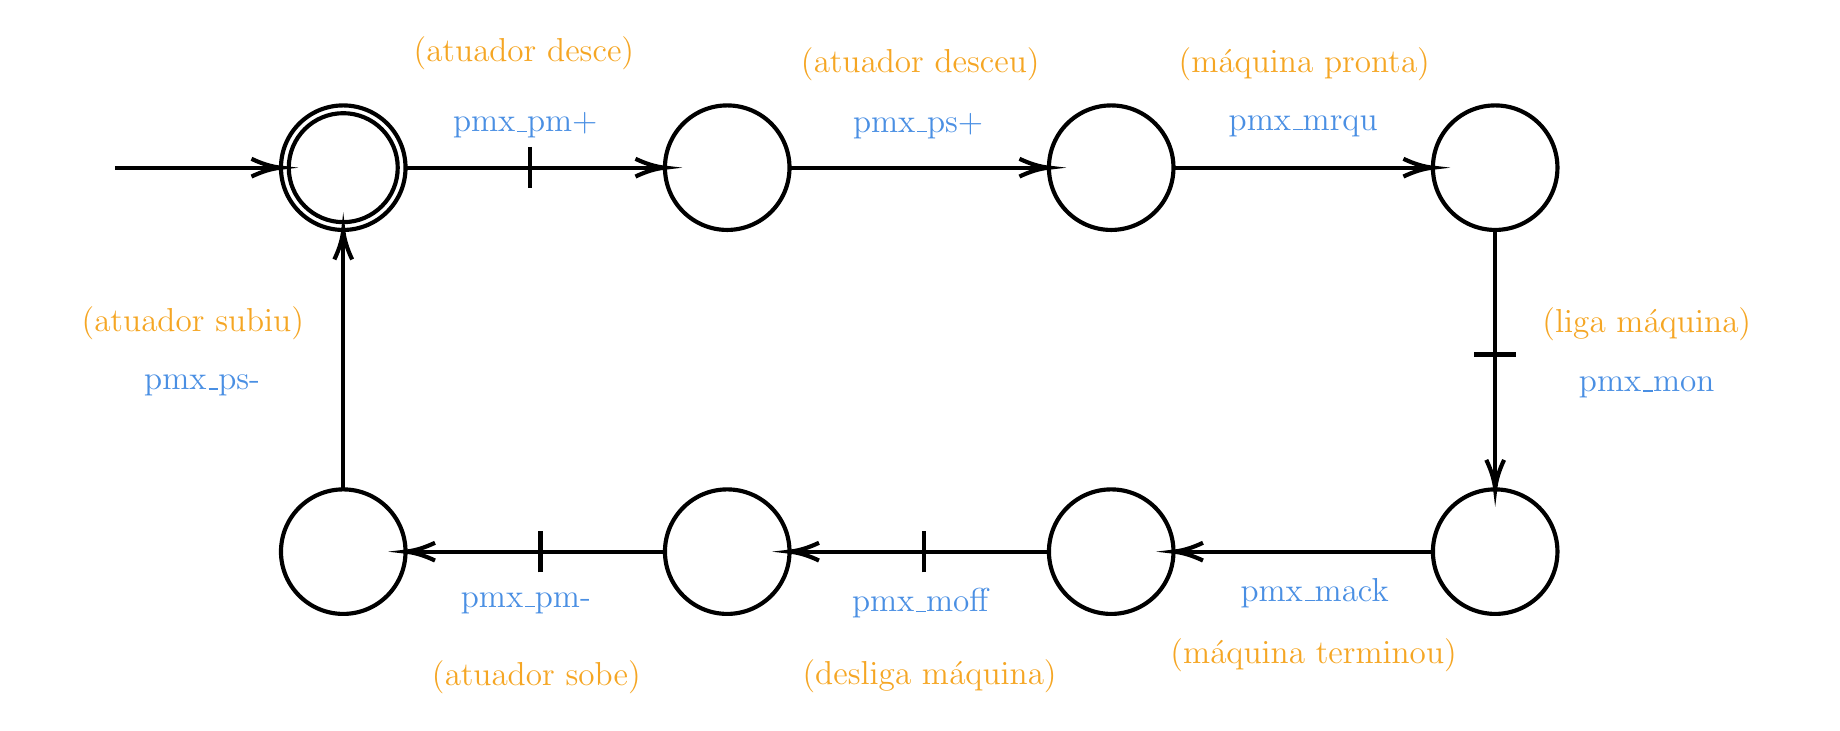
\begin{tikzpicture}[x=0.75pt,y=0.75pt,yscale=-1,xscale=1]
%uncomment if require: \path (0,3420); %set diagram left start at 0, and has height of 3420

%Shape: Circle [id:dp03983393294822668] 
\draw  [line width=1.5]  (195,570) .. controls (195,553.43) and (208.43,540) .. (225,540) .. controls (241.57,540) and (255,553.43) .. (255,570) .. controls (255,586.57) and (241.57,600) .. (225,600) .. controls (208.43,600) and (195,586.57) .. (195,570) -- cycle ;
%Shape: Circle [id:dp5386939635952754] 
\draw  [line width=1.5]  (198.75,570) .. controls (198.75,555.5) and (210.5,543.75) .. (225,543.75) .. controls (239.5,543.75) and (251.25,555.5) .. (251.25,570) .. controls (251.25,584.5) and (239.5,596.25) .. (225,596.25) .. controls (210.5,596.25) and (198.75,584.5) .. (198.75,570) -- cycle ;
%Straight Lines [id:da7472247027350285] 
\draw [line width=1.5]    (115,570) -- (192,570) ;
\draw [shift={(195,570)}, rotate = 180] [color={rgb, 255:red, 0; green, 0; blue, 0 }  ][line width=1.5]    (14.21,-4.28) .. controls (9.04,-1.82) and (4.3,-0.39) .. (0,0) .. controls (4.3,0.39) and (9.04,1.82) .. (14.21,4.28)   ;
%Straight Lines [id:da7245864288717945] 
\draw [line width=1.5]    (255,570) -- (278,570) -- (377,570) ;
\draw [shift={(380,570)}, rotate = 180] [color={rgb, 255:red, 0; green, 0; blue, 0 }  ][line width=1.5]    (14.21,-4.28) .. controls (9.04,-1.82) and (4.3,-0.39) .. (0,0) .. controls (4.3,0.39) and (9.04,1.82) .. (14.21,4.28)   ;
%Straight Lines [id:da4408332158733741] 
\draw [line width=1.5]    (315,560) -- (315,580) ;

%Shape: Circle [id:dp7756612921759896] 
\draw  [line width=1.5]  (380,570) .. controls (380,553.43) and (393.43,540) .. (410,540) .. controls (426.57,540) and (440,553.43) .. (440,570) .. controls (440,586.57) and (426.57,600) .. (410,600) .. controls (393.43,600) and (380,586.57) .. (380,570) -- cycle ;
%Straight Lines [id:da31825762072206665] 
\draw [line width=1.5]    (440,570) -- (562,570) ;
\draw [shift={(565,570)}, rotate = 180] [color={rgb, 255:red, 0; green, 0; blue, 0 }  ][line width=1.5]    (14.21,-4.28) .. controls (9.04,-1.82) and (4.3,-0.39) .. (0,0) .. controls (4.3,0.39) and (9.04,1.82) .. (14.21,4.28)   ;
%Shape: Circle [id:dp7372149376145194] 
\draw  [line width=1.5]  (565,570) .. controls (565,553.43) and (578.43,540) .. (595,540) .. controls (611.57,540) and (625,553.43) .. (625,570) .. controls (625,586.57) and (611.57,600) .. (595,600) .. controls (578.43,600) and (565,586.57) .. (565,570) -- cycle ;
%Straight Lines [id:da9364368992463274] 
\draw [line width=1.5]    (625,570) -- (747,570) ;
\draw [shift={(750,570)}, rotate = 180] [color={rgb, 255:red, 0; green, 0; blue, 0 }  ][line width=1.5]    (14.21,-4.28) .. controls (9.04,-1.82) and (4.3,-0.39) .. (0,0) .. controls (4.3,0.39) and (9.04,1.82) .. (14.21,4.28)   ;
%Shape: Circle [id:dp3065440607390728] 
\draw  [line width=1.5]  (750,570) .. controls (750,553.43) and (763.43,540) .. (780,540) .. controls (796.57,540) and (810,553.43) .. (810,570) .. controls (810,586.57) and (796.57,600) .. (780,600) .. controls (763.43,600) and (750,586.57) .. (750,570) -- cycle ;
%Straight Lines [id:da46216885822973097] 
\draw [line width=1.5]    (780,600) -- (780,623) -- (780,722) ;
\draw [shift={(780,725)}, rotate = 270] [color={rgb, 255:red, 0; green, 0; blue, 0 }  ][line width=1.5]    (14.21,-4.28) .. controls (9.04,-1.82) and (4.3,-0.39) .. (0,0) .. controls (4.3,0.39) and (9.04,1.82) .. (14.21,4.28)   ;
%Straight Lines [id:da24276305465802062] 
\draw [line width=1.5]    (790,660) -- (770,660) ;

%Shape: Circle [id:dp6769316860879337] 
\draw  [line width=1.5]  (750,755) .. controls (750,738.43) and (763.43,725) .. (780,725) .. controls (796.57,725) and (810,738.43) .. (810,755) .. controls (810,771.57) and (796.57,785) .. (780,785) .. controls (763.43,785) and (750,771.57) .. (750,755) -- cycle ;
%Straight Lines [id:da21528525866552095] 
\draw [line width=1.5]    (628,755) -- (750,755) ;
\draw [shift={(625,755)}, rotate = 0] [color={rgb, 255:red, 0; green, 0; blue, 0 }  ][line width=1.5]    (14.21,-4.28) .. controls (9.04,-1.82) and (4.3,-0.39) .. (0,0) .. controls (4.3,0.39) and (9.04,1.82) .. (14.21,4.28)   ;
%Shape: Circle [id:dp5763603692577981] 
\draw  [line width=1.5]  (565,755) .. controls (565,738.43) and (578.43,725) .. (595,725) .. controls (611.57,725) and (625,738.43) .. (625,755) .. controls (625,771.57) and (611.57,785) .. (595,785) .. controls (578.43,785) and (565,771.57) .. (565,755) -- cycle ;
%Shape: Circle [id:dp604112390985414] 
\draw  [line width=1.5]  (380,755) .. controls (380,738.43) and (393.43,725) .. (410,725) .. controls (426.57,725) and (440,738.43) .. (440,755) .. controls (440,771.57) and (426.57,785) .. (410,785) .. controls (393.43,785) and (380,771.57) .. (380,755) -- cycle ;
%Shape: Circle [id:dp12255566070328827] 
\draw  [line width=1.5]  (195,755) .. controls (195,738.43) and (208.43,725) .. (225,725) .. controls (241.57,725) and (255,738.43) .. (255,755) .. controls (255,771.57) and (241.57,785) .. (225,785) .. controls (208.43,785) and (195,771.57) .. (195,755) -- cycle ;
%Straight Lines [id:da3455914070693218] 
\draw [line width=1.5]    (565,755) -- (542,755) -- (443,755) ;
\draw [shift={(440,755)}, rotate = 360] [color={rgb, 255:red, 0; green, 0; blue, 0 }  ][line width=1.5]    (14.21,-4.28) .. controls (9.04,-1.82) and (4.3,-0.39) .. (0,0) .. controls (4.3,0.39) and (9.04,1.82) .. (14.21,4.28)   ;
%Straight Lines [id:da717285302912293] 
\draw [line width=1.5]    (505,765) -- (505,745) ;

%Straight Lines [id:da5597257425893609] 
\draw [line width=1.5]    (380,755) -- (357,755) -- (258,755) ;
\draw [shift={(255,755)}, rotate = 360] [color={rgb, 255:red, 0; green, 0; blue, 0 }  ][line width=1.5]    (14.21,-4.28) .. controls (9.04,-1.82) and (4.3,-0.39) .. (0,0) .. controls (4.3,0.39) and (9.04,1.82) .. (14.21,4.28)   ;
%Straight Lines [id:da5009808196347338] 
\draw [line width=1.5]    (320,765) -- (320,745) ;

%Shape: Boxed Line [id:dp30413583145545564] 
\draw [line width=1.5]    (225,725) -- (225,603) ;
\draw [shift={(225,600)}, rotate = 90] [color={rgb, 255:red, 0; green, 0; blue, 0 }  ][line width=1.5]    (14.21,-4.28) .. controls (9.04,-1.82) and (4.3,-0.39) .. (0,0) .. controls (4.3,0.39) and (9.04,1.82) .. (14.21,4.28)   ;

% Text Node
\draw (312,545) node  [font=\large] [align=left] {\begin{minipage}[lt]{51.17pt}\setlength\topsep{0pt}
\begin{center}
\textcolor[rgb]{0.29,0.56,0.89}{pmx\_pm+}
\end{center}

\end{minipage}};
% Text Node
\draw (312,515) node  [font=\large] [align=left] {\begin{minipage}[lt]{91.55pt}\setlength\topsep{0pt}
\begin{center}
\textcolor[rgb]{0.96,0.65,0.14}{(atuador desce)}
\end{center}

\end{minipage}};
% Text Node
\draw (502,550) node  [font=\large] [align=left] {\begin{minipage}[lt]{51.17pt}\setlength\topsep{0pt}
\begin{center}
\textcolor[rgb]{0.29,0.56,0.89}{pmx\_ps+}
\end{center}

\end{minipage}};
% Text Node
\draw (503,520) node  [font=\large] [align=left] {\begin{minipage}[lt]{98.81pt}\setlength\topsep{0pt}
\begin{center}
\textcolor[rgb]{0.96,0.65,0.14}{(atuador desceu)}
\end{center}

\end{minipage}};
% Text Node
\draw (687.5,550) node  [font=\large] [align=left] {\begin{minipage}[lt]{58.23pt}\setlength\topsep{0pt}
\begin{center}
\textcolor[rgb]{0.29,0.56,0.89}{pmx\_mrqu}
\end{center}

\end{minipage}};
% Text Node
\draw (688,520) node  [font=\large] [align=left] {\begin{minipage}[lt]{98.81pt}\setlength\topsep{0pt}
\begin{center}
\textcolor[rgb]{0.96,0.65,0.14}{(máquina pronta)}
\end{center}

\end{minipage}};
% Text Node
\draw (693,775) node  [font=\large] [align=left] {\begin{minipage}[lt]{57.55pt}\setlength\topsep{0pt}
\begin{center}
\textcolor[rgb]{0.29,0.56,0.89}{pmx\_mack}
\end{center}

\end{minipage}};
% Text Node
\draw (692.5,805) node  [font=\large] [align=left] {\begin{minipage}[lt]{112.65pt}\setlength\topsep{0pt}
\begin{center}
\textcolor[rgb]{0.96,0.65,0.14}{(máquina terminou)}
\end{center}

\end{minipage}};
% Text Node
\draw (853,676) node  [font=\large] [align=left] {\begin{minipage}[lt]{57.55pt}\setlength\topsep{0pt}
\begin{center}
\textcolor[rgb]{0.29,0.56,0.89}{pmx\_mon}
\end{center}

\end{minipage}};
% Text Node
\draw (853,645.5) node  [font=\large] [align=left] {\begin{minipage}[lt]{112.65pt}\setlength\topsep{0pt}
\begin{center}
\textcolor[rgb]{0.96,0.65,0.14}{(liga máquina)}
\end{center}

\end{minipage}};
% Text Node
\draw (503,780) node  [font=\large] [align=left] {\begin{minipage}[lt]{57.55pt}\setlength\topsep{0pt}
\begin{center}
\textcolor[rgb]{0.29,0.56,0.89}{pmx\_moff}
\end{center}

\end{minipage}};
% Text Node
\draw (507.5,815) node  [font=\large] [align=left] {\begin{minipage}[lt]{112.65pt}\setlength\topsep{0pt}
\begin{center}
\textcolor[rgb]{0.96,0.65,0.14}{(desliga máquina)}
\end{center}

\end{minipage}};
% Text Node
\draw (313,780) node  [font=\large] [align=left] {\begin{minipage}[lt]{57.55pt}\setlength\topsep{0pt}
\begin{center}
\textcolor[rgb]{0.29,0.56,0.89}{pmx\_pm-}
\end{center}

\end{minipage}};
% Text Node
\draw (318,815.5) node  [font=\large] [align=left] {\begin{minipage}[lt]{112.65pt}\setlength\topsep{0pt}
\begin{center}
\textcolor[rgb]{0.96,0.65,0.14}{(atuador sobe)}
\end{center}

\end{minipage}};
% Text Node
\draw (157,675) node  [font=\large] [align=left] {\begin{minipage}[lt]{57.55pt}\setlength\topsep{0pt}
\begin{center}
\textcolor[rgb]{0.29,0.56,0.89}{pmx\_ps-}
\end{center}

\end{minipage}};
% Text Node
\draw (152.5,645) node  [font=\large] [align=left] {\begin{minipage}[lt]{112.65pt}\setlength\topsep{0pt}
\begin{center}
\textcolor[rgb]{0.96,0.65,0.14}{(atuador subiu)}
\end{center}

\end{minipage}};


\end{tikzpicture}}
        \caption{\textbf{Atuador} do \textit{processing machine}.}
        \label{fig:sistema}
    \end{figure}
    \textbf{OBS.:} o $x$ em cada sinal representa qual a máquina em questão: 1 ou 2.
\end{frame}
\begin{frame}{\textit{Processing Machine} (PM1 e PM2)}
    \begin{figure}[htbp]
        \centering
        \resizebox{0.9\textwidth}{!}{


\tikzset{every picture/.style={line width=0.75pt}} %set default line width to 0.75pt        

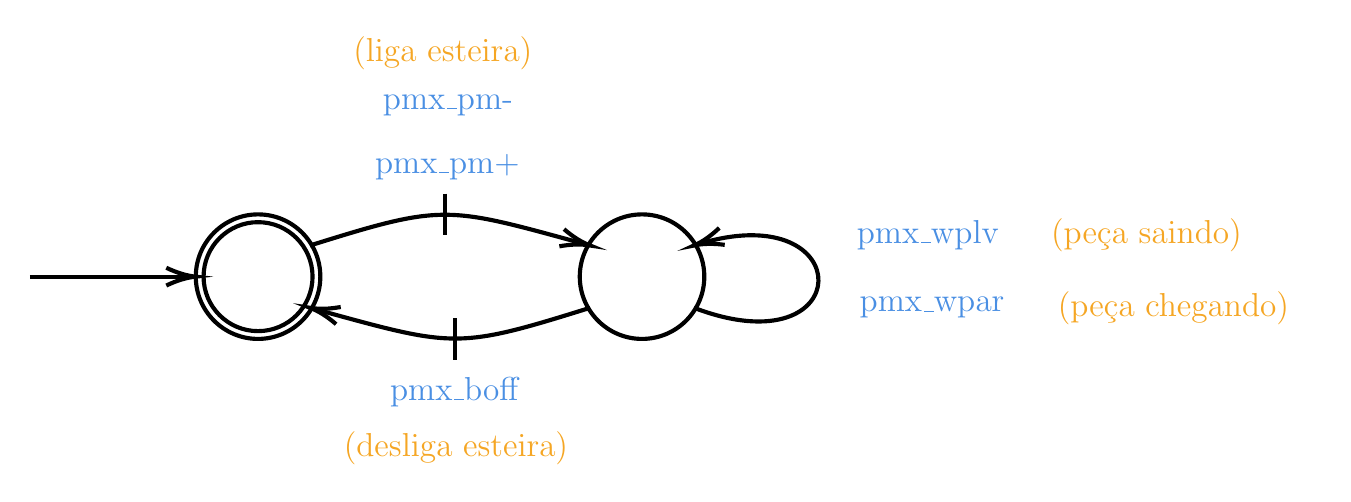
\begin{tikzpicture}[x=0.75pt,y=0.75pt,yscale=-1,xscale=1]
%uncomment if require: \path (0,1382); %set diagram left start at 0, and has height of 1382

%Shape: Circle [id:dp7056372270075382] 
\draw  [line width=1.5]  (200,990) .. controls (200,973.43) and (213.43,960) .. (230,960) .. controls (246.57,960) and (260,973.43) .. (260,990) .. controls (260,1006.57) and (246.57,1020) .. (230,1020) .. controls (213.43,1020) and (200,1006.57) .. (200,990) -- cycle ;
%Shape: Circle [id:dp7389265971510601] 
\draw  [line width=1.5]  (203.75,990) .. controls (203.75,975.5) and (215.5,963.75) .. (230,963.75) .. controls (244.5,963.75) and (256.25,975.5) .. (256.25,990) .. controls (256.25,1004.5) and (244.5,1016.25) .. (230,1016.25) .. controls (215.5,1016.25) and (203.75,1004.5) .. (203.75,990) -- cycle ;
%Straight Lines [id:da8531216177666909] 
\draw [line width=1.5]    (120,990) -- (197,990) ;
\draw [shift={(200,990)}, rotate = 180] [color={rgb, 255:red, 0; green, 0; blue, 0 }  ][line width=1.5]    (14.21,-4.28) .. controls (9.04,-1.82) and (4.3,-0.39) .. (0,0) .. controls (4.3,0.39) and (9.04,1.82) .. (14.21,4.28)   ;
%Straight Lines [id:da8917004523902834] 
\draw [line width=1.5]    (320,950) -- (320,970) ;
%Shape: Circle [id:dp6571331930145972] 
\draw  [line width=1.5]  (385,990) .. controls (385,973.43) and (398.43,960) .. (415,960) .. controls (431.57,960) and (445,973.43) .. (445,990) .. controls (445,1006.57) and (431.57,1020) .. (415,1020) .. controls (398.43,1020) and (385,1006.57) .. (385,990) -- cycle ;
%Curve Lines [id:da8046766398483354] 
\draw [line width=1.5]    (255,975) .. controls (319.85,954.71) and (320.49,955.97) .. (387.94,974.44) ;
\draw [shift={(390,975)}, rotate = 195.29] [color={rgb, 255:red, 0; green, 0; blue, 0 }  ][line width=1.5]    (14.21,-4.28) .. controls (9.04,-1.82) and (4.3,-0.39) .. (0,0) .. controls (4.3,0.39) and (9.04,1.82) .. (14.21,4.28)   ;
%Straight Lines [id:da8168460983392734] 
\draw [line width=1.5]    (325,1030) -- (325,1010) ;
%Curve Lines [id:da4505905673241448] 
\draw [line width=1.5]    (390,1005) .. controls (325.15,1025.3) and (324.51,1024.03) .. (257.06,1005.56) ;
\draw [shift={(255,1005)}, rotate = 15.29] [color={rgb, 255:red, 0; green, 0; blue, 0 }  ][line width=1.5]    (14.21,-4.28) .. controls (9.04,-1.82) and (4.3,-0.39) .. (0,0) .. controls (4.3,0.39) and (9.04,1.82) .. (14.21,4.28)   ;

%Curve Lines [id:da3095367406252396] 
\draw [line width=1.5]    (440,1005) .. controls (519.2,1035.2) and (519.99,950.72) .. (442.38,974.25) ;
\draw [shift={(440,975)}, rotate = 342] [color={rgb, 255:red, 0; green, 0; blue, 0 }  ][line width=1.5]    (14.21,-4.28) .. controls (9.04,-1.82) and (4.3,-0.39) .. (0,0) .. controls (4.3,0.39) and (9.04,1.82) .. (14.21,4.28)   ;

% Text Node
\draw (320.5,932.5) node  [font=\large] [align=left] {\begin{minipage}[lt]{51.17pt}\setlength\topsep{0pt}
\begin{center}
\textcolor[rgb]{0.29,0.56,0.89}{pmx\_pm+}
\end{center}

\end{minipage}};
% Text Node
\draw (319,882.5) node  [font=\large] [align=left] {\begin{minipage}[lt]{91.55pt}\setlength\topsep{0pt}
\begin{center}
\textcolor[rgb]{0.96,0.65,0.14}{(liga esteira)}
\end{center}

\end{minipage}};
% Text Node
\draw (321.5,907.5) node  [font=\large] [align=left] {\begin{minipage}[lt]{51.17pt}\setlength\topsep{0pt}
\begin{center}
\textcolor[rgb]{0.29,0.56,0.89}{pmx\_pm-}
\end{center}

\end{minipage}};
% Text Node
\draw (325.34,1072.5) node  [font=\large] [align=left] {\begin{minipage}[lt]{98.13pt}\setlength\topsep{0pt}
\begin{center}
\textcolor[rgb]{0.96,0.65,0.14}{(desliga esteira)}
\end{center}

\end{minipage}};
% Text Node
\draw (324.5,1045.5) node  [font=\large] [align=left] {\begin{minipage}[lt]{51.17pt}\setlength\topsep{0pt}
\begin{center}
\textcolor[rgb]{0.29,0.56,0.89}{pmx\_boff}
\end{center}

\end{minipage}};
% Text Node
\draw (552.69,970) node  [font=\large] [align=left] {\begin{minipage}[lt]{57.55pt}\setlength\topsep{0pt}
\begin{center}
\textcolor[rgb]{0.29,0.56,0.89}{pmx\_wplv}
\end{center}

\end{minipage}};
% Text Node
\draw (658,970) node  [font=\large] [align=left] {\begin{minipage}[lt]{91.55pt}\setlength\topsep{0pt}
\begin{center}
\textcolor[rgb]{0.96,0.65,0.14}{(peça saindo)}
\end{center}

\end{minipage}};
% Text Node
\draw (554.69,1005) node  [font=\large] [align=left] {\begin{minipage}[lt]{61.63pt}\setlength\topsep{0pt}
\begin{center}
\textcolor[rgb]{0.29,0.56,0.89}{pmx\_wpar}
\end{center}

\end{minipage}};
% Text Node
\draw (671,1005) node  [font=\large] [align=left] {\begin{minipage}[lt]{101.53pt}\setlength\topsep{0pt}
\begin{center}
\textcolor[rgb]{0.96,0.65,0.14}{(peça chegando)}
\end{center}

\end{minipage}};


\end{tikzpicture}}
        \caption{\textbf{Esteira} do \textit{processing machine}.}
        \label{fig:sistema}
    \end{figure}
    \textbf{OBS.:} o $x$ em cada sinal representa qual a máquina em questão: 1 ou 2.
\end{frame}
\begin{frame}{\textit{Stack Feeder} (SF)}
    \begin{figure}[htbp]
        \centering
        \resizebox{0.65\textwidth}{!}{


\tikzset{every picture/.style={line width=0.75pt}} %set default line width to 0.75pt        

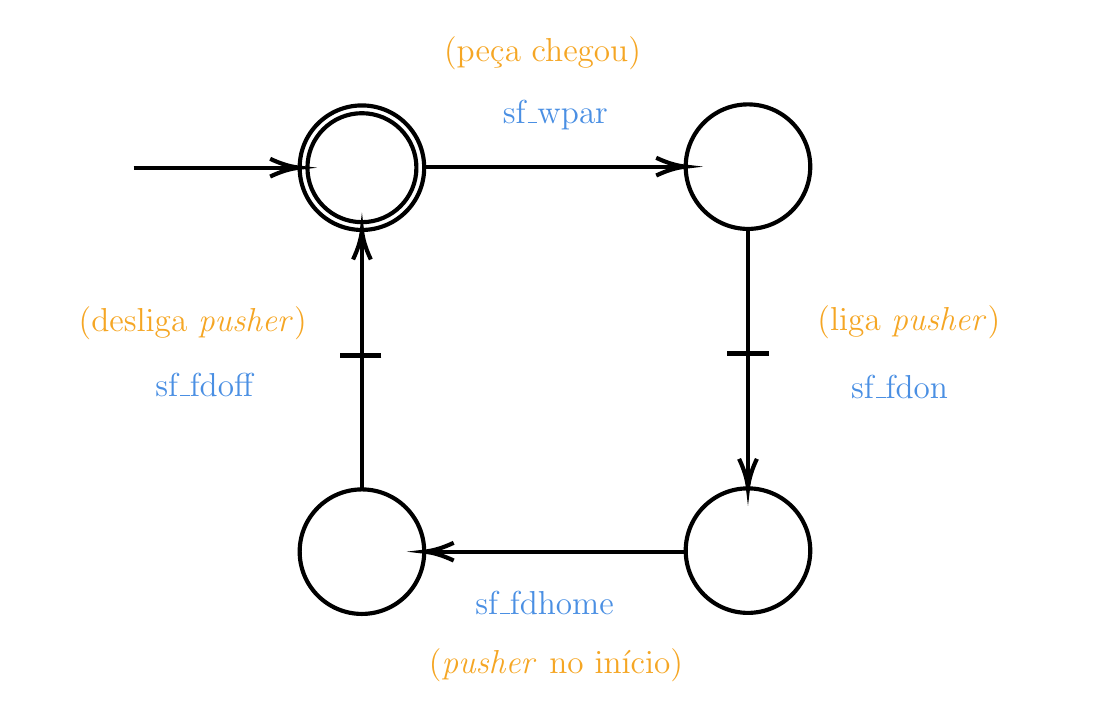
\begin{tikzpicture}[x=0.75pt,y=0.75pt,yscale=-1,xscale=1]
%uncomment if require: \path (0,1950); %set diagram left start at 0, and has height of 1950

%Shape: Circle [id:dp9519934708871869] 
\draw  [line width=1.5]  (199,1195.5) .. controls (199,1178.93) and (212.43,1165.5) .. (229,1165.5) .. controls (245.57,1165.5) and (259,1178.93) .. (259,1195.5) .. controls (259,1212.07) and (245.57,1225.5) .. (229,1225.5) .. controls (212.43,1225.5) and (199,1212.07) .. (199,1195.5) -- cycle ;
%Shape: Circle [id:dp32256561980977216] 
\draw  [line width=1.5]  (202.75,1195.5) .. controls (202.75,1181) and (214.5,1169.25) .. (229,1169.25) .. controls (243.5,1169.25) and (255.25,1181) .. (255.25,1195.5) .. controls (255.25,1210) and (243.5,1221.75) .. (229,1221.75) .. controls (214.5,1221.75) and (202.75,1210) .. (202.75,1195.5) -- cycle ;
%Straight Lines [id:da9013209386358128] 
\draw [line width=1.5]    (119,1195.5) -- (196,1195.5) ;
\draw [shift={(199,1195.5)}, rotate = 180] [color={rgb, 255:red, 0; green, 0; blue, 0 }  ][line width=1.5]    (14.21,-4.28) .. controls (9.04,-1.82) and (4.3,-0.39) .. (0,0) .. controls (4.3,0.39) and (9.04,1.82) .. (14.21,4.28)   ;
%Straight Lines [id:da39365127810115874] 
\draw [line width=1.5]    (260,1195) -- (283,1195) -- (382,1195) ;
\draw [shift={(385,1195)}, rotate = 180] [color={rgb, 255:red, 0; green, 0; blue, 0 }  ][line width=1.5]    (14.21,-4.28) .. controls (9.04,-1.82) and (4.3,-0.39) .. (0,0) .. controls (4.3,0.39) and (9.04,1.82) .. (14.21,4.28)   ;
%Shape: Circle [id:dp25396435792249483] 
\draw  [line width=1.5]  (385,1195) .. controls (385,1178.43) and (398.43,1165) .. (415,1165) .. controls (431.57,1165) and (445,1178.43) .. (445,1195) .. controls (445,1211.57) and (431.57,1225) .. (415,1225) .. controls (398.43,1225) and (385,1211.57) .. (385,1195) -- cycle ;
%Straight Lines [id:da8766626537212896] 
\draw [line width=1.5]    (415,1225) -- (415,1248) -- (415,1347) ;
\draw [shift={(415,1350)}, rotate = 270] [color={rgb, 255:red, 0; green, 0; blue, 0 }  ][line width=1.5]    (14.21,-4.28) .. controls (9.04,-1.82) and (4.3,-0.39) .. (0,0) .. controls (4.3,0.39) and (9.04,1.82) .. (14.21,4.28)   ;
%Straight Lines [id:da841229893246316] 
\draw [line width=1.5]    (425,1285) -- (405,1285) ;

%Shape: Circle [id:dp6492238720051349] 
\draw  [line width=1.5]  (385,1380) .. controls (385,1363.43) and (398.43,1350) .. (415,1350) .. controls (431.57,1350) and (445,1363.43) .. (445,1380) .. controls (445,1396.57) and (431.57,1410) .. (415,1410) .. controls (398.43,1410) and (385,1396.57) .. (385,1380) -- cycle ;
%Shape: Circle [id:dp8616591257447523] 
\draw  [line width=1.5]  (199,1380.5) .. controls (199,1363.93) and (212.43,1350.5) .. (229,1350.5) .. controls (245.57,1350.5) and (259,1363.93) .. (259,1380.5) .. controls (259,1397.07) and (245.57,1410.5) .. (229,1410.5) .. controls (212.43,1410.5) and (199,1397.07) .. (199,1380.5) -- cycle ;
%Straight Lines [id:da04524750371954256] 
\draw [line width=1.5]    (384,1380.5) -- (361,1380.5) -- (262,1380.5) ;
\draw [shift={(259,1380.5)}, rotate = 360] [color={rgb, 255:red, 0; green, 0; blue, 0 }  ][line width=1.5]    (14.21,-4.28) .. controls (9.04,-1.82) and (4.3,-0.39) .. (0,0) .. controls (4.3,0.39) and (9.04,1.82) .. (14.21,4.28)   ;
%Straight Lines [id:da7226466086806207] 
\draw [line width=1.5]    (238.4,1286) -- (218.4,1286) ;
%Shape: Boxed Line [id:dp04703168518726075] 
\draw [line width=1.5]    (229,1350.5) -- (229,1228.5) ;
\draw [shift={(229,1225.5)}, rotate = 90] [color={rgb, 255:red, 0; green, 0; blue, 0 }  ][line width=1.5]    (14.21,-4.28) .. controls (9.04,-1.82) and (4.3,-0.39) .. (0,0) .. controls (4.3,0.39) and (9.04,1.82) .. (14.21,4.28)   ;

% Text Node
\draw (322.19,1170) node  [font=\large] [align=left] {\begin{minipage}[lt]{58.23pt}\setlength\topsep{0pt}
\begin{center}
\textcolor[rgb]{0.29,0.56,0.89}{sf\_wpar}
\end{center}

\end{minipage}};
% Text Node
\draw (316,1140.5) node  [font=\large] [align=left] {\begin{minipage}[lt]{91.55pt}\setlength\topsep{0pt}
\begin{center}
\textcolor[rgb]{0.96,0.65,0.14}{(peça chegou)}
\end{center}

\end{minipage}};
% Text Node
\draw (488,1301) node  [font=\large] [align=left] {\begin{minipage}[lt]{57.55pt}\setlength\topsep{0pt}
\begin{center}
\textcolor[rgb]{0.29,0.56,0.89}{sf\_fdon}
\end{center}

\end{minipage}};
% Text Node
\draw (492.5,1270) node  [font=\large] [align=left] {\begin{minipage}[lt]{112.65pt}\setlength\topsep{0pt}
\begin{center}
\textcolor[rgb]{0.96,0.65,0.14}{(liga \textit{pusher})}
\end{center}

\end{minipage}};
% Text Node
\draw (317,1405) node  [font=\large] [align=left] {\begin{minipage}[lt]{57.55pt}\setlength\topsep{0pt}
\begin{center}
\textcolor[rgb]{0.29,0.56,0.89}{sf\_fdhome}
\end{center}

\end{minipage}};
% Text Node
\draw (322.5,1435) node  [font=\large] [align=left] {\begin{minipage}[lt]{112.65pt}\setlength\topsep{0pt}
\begin{center}
\textcolor[rgb]{0.96,0.65,0.14}{(\textit{pusher }no início)}
\end{center}

\end{minipage}};
% Text Node
\draw (153,1300) node  [font=\large] [align=left] {\begin{minipage}[lt]{57.55pt}\setlength\topsep{0pt}
\begin{center}
\textcolor[rgb]{0.29,0.56,0.89}{sf\_fdoff}
\end{center}

\end{minipage}};
% Text Node
\draw (147.5,1270.5) node  [font=\large] [align=left] {\begin{minipage}[lt]{112.65pt}\setlength\topsep{0pt}
\begin{center}
\textcolor[rgb]{0.96,0.65,0.14}{(desliga \textit{pusher})}
\end{center}

\end{minipage}};


\end{tikzpicture}}
        \caption{\textit{Stack feeder} completo.}
        \label{fig:sistema}
    \end{figure}
\end{frame}
\begin{frame}{\textit{Exit Slide} (XS)}
    \begin{figure}[htbp]
        \centering
        \resizebox{0.45\textwidth}{!}{


\tikzset{every picture/.style={line width=0.75pt}} %set default line width to 0.75pt        

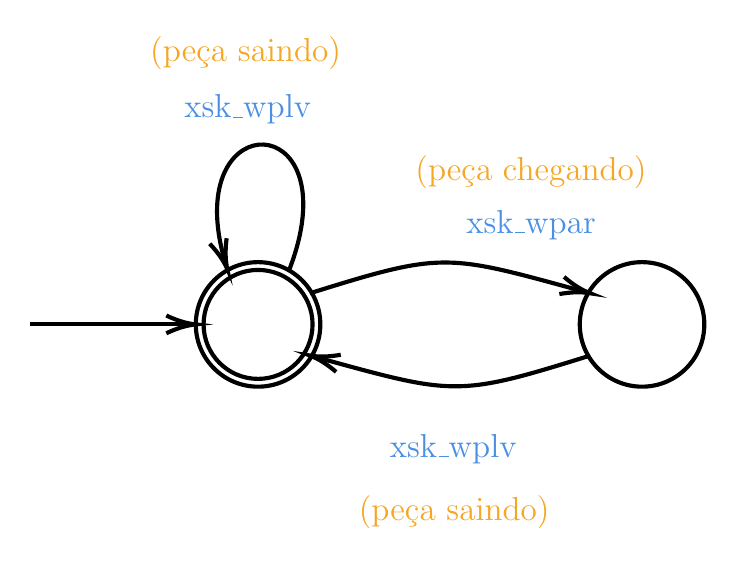
\begin{tikzpicture}[x=0.75pt,y=0.75pt,yscale=-1,xscale=1]
%uncomment if require: \path (0,1950); %set diagram left start at 0, and has height of 1950

%Shape: Circle [id:dp022173602878892806] 
\draw  [line width=1.5]  (190,1647) .. controls (190,1630.43) and (203.43,1617) .. (220,1617) .. controls (236.57,1617) and (250,1630.43) .. (250,1647) .. controls (250,1663.57) and (236.57,1677) .. (220,1677) .. controls (203.43,1677) and (190,1663.57) .. (190,1647) -- cycle ;
%Shape: Circle [id:dp423715485375872] 
\draw  [line width=1.5]  (193.75,1647) .. controls (193.75,1632.5) and (205.5,1620.75) .. (220,1620.75) .. controls (234.5,1620.75) and (246.25,1632.5) .. (246.25,1647) .. controls (246.25,1661.5) and (234.5,1673.25) .. (220,1673.25) .. controls (205.5,1673.25) and (193.75,1661.5) .. (193.75,1647) -- cycle ;
%Straight Lines [id:da5144723553129629] 
\draw [line width=1.5]    (110,1647) -- (187,1647) ;
\draw [shift={(190,1647)}, rotate = 180] [color={rgb, 255:red, 0; green, 0; blue, 0 }  ][line width=1.5]    (14.21,-4.28) .. controls (9.04,-1.82) and (4.3,-0.39) .. (0,0) .. controls (4.3,0.39) and (9.04,1.82) .. (14.21,4.28)   ;
%Shape: Circle [id:dp4674994120096958] 
\draw  [line width=1.5]  (375,1647) .. controls (375,1630.43) and (388.43,1617) .. (405,1617) .. controls (421.57,1617) and (435,1630.43) .. (435,1647) .. controls (435,1663.57) and (421.57,1677) .. (405,1677) .. controls (388.43,1677) and (375,1663.57) .. (375,1647) -- cycle ;
%Curve Lines [id:da004365420011859467] 
\draw [line width=1.5]    (245,1632) .. controls (309.85,1611.71) and (310.49,1612.97) .. (377.94,1631.44) ;
\draw [shift={(380,1632)}, rotate = 195.29] [color={rgb, 255:red, 0; green, 0; blue, 0 }  ][line width=1.5]    (14.21,-4.28) .. controls (9.04,-1.82) and (4.3,-0.39) .. (0,0) .. controls (4.3,0.39) and (9.04,1.82) .. (14.21,4.28)   ;
%Curve Lines [id:da7829654720886046] 
\draw [line width=1.5]    (380,1662) .. controls (315.15,1682.3) and (314.51,1681.03) .. (247.06,1662.56) ;
\draw [shift={(245,1662)}, rotate = 15.29] [color={rgb, 255:red, 0; green, 0; blue, 0 }  ][line width=1.5]    (14.21,-4.28) .. controls (9.04,-1.82) and (4.3,-0.39) .. (0,0) .. controls (4.3,0.39) and (9.04,1.82) .. (14.21,4.28)   ;
%Shape: Boxed Bezier Curve [id:dp8439384559463989] 
\draw [line width=1.5]    (235.17,1620.33) .. controls (263.28,1546.6) and (192.01,1540.82) .. (201.02,1602.99) .. controls (201.67,1607.49) and (202.74,1612.34) .. (204.3,1617.54) ;
\draw [shift={(205.17,1620.33)}, rotate = 252] [color={rgb, 255:red, 0; green, 0; blue, 0 }  ][line width=1.5]    (14.21,-4.28) .. controls (9.04,-1.82) and (4.3,-0.39) .. (0,0) .. controls (4.3,0.39) and (9.04,1.82) .. (14.21,4.28)   ;

% Text Node
\draw (351.5,1599) node  [font=\large] [align=left] {\begin{minipage}[lt]{51.17pt}\setlength\topsep{0pt}
\begin{center}
\textcolor[rgb]{0.29,0.56,0.89}{xsk\_wpar}
\end{center}

\end{minipage}};
% Text Node
\draw (314.5,1737.5) node  [font=\large] [align=left] {\begin{minipage}[lt]{91.55pt}\setlength\topsep{0pt}
\begin{center}
\textcolor[rgb]{0.96,0.65,0.14}{(peça saindo)}
\end{center}

\end{minipage}};
% Text Node
\draw (351.5,1573.5) node  [font=\large] [align=left] {\begin{minipage}[lt]{101.53pt}\setlength\topsep{0pt}
\begin{center}
\textcolor[rgb]{0.96,0.65,0.14}{(peça chegando)}
\end{center}

\end{minipage}};
% Text Node
\draw (314,1707) node  [font=\large] [align=left] {\begin{minipage}[lt]{51.17pt}\setlength\topsep{0pt}
\begin{center}
\textcolor[rgb]{0.29,0.56,0.89}{xsk\_wplv}
\end{center}

\end{minipage}};
% Text Node
\draw (215,1543.5) node  [font=\large] [align=left] {\begin{minipage}[lt]{51.17pt}\setlength\topsep{0pt}
\begin{center}
\textcolor[rgb]{0.29,0.56,0.89}{xsk\_wplv}
\end{center}

\end{minipage}};
% Text Node
\draw (214,1516.5) node  [font=\large] [align=left] {\begin{minipage}[lt]{91.55pt}\setlength\topsep{0pt}
\begin{center}
\textcolor[rgb]{0.96,0.65,0.14}{(peça saindo)}
\end{center}

\end{minipage}};


\end{tikzpicture}}
        \caption{\textit{Exit slide} completo.}
        \label{fig:sistema}
    \end{figure}
    \textbf{OBS.:} o $k$ em cada sinal representa qual a máquina em questão: 1 ou 2.
\end{frame}
\begin{frame}{\textit{Distribution System} (DS)}
    \begin{figure}[htbp]
        \centering
        \resizebox{1\textwidth}{!}{


\tikzset{every picture/.style={line width=0.75pt}} %set default line width to 0.75pt        

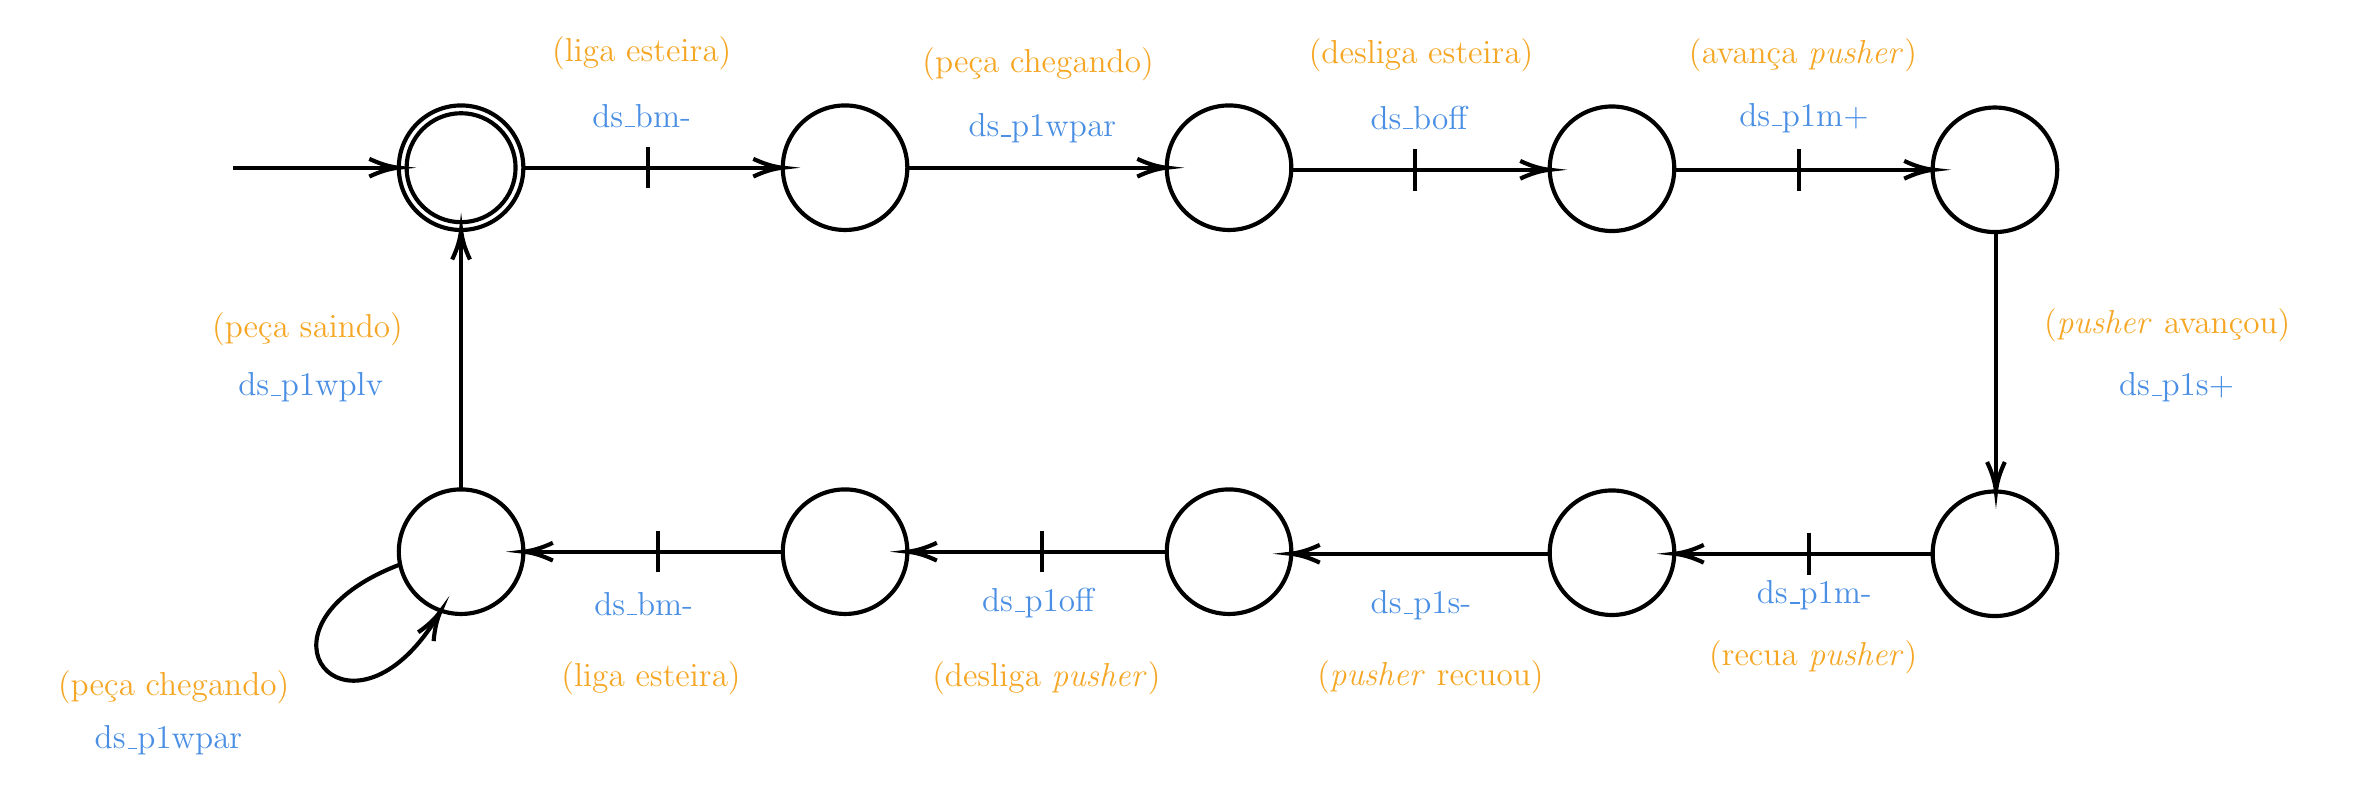
\begin{tikzpicture}[x=0.75pt,y=0.75pt,yscale=-1,xscale=1]
%uncomment if require: \path (0,2709); %set diagram left start at 0, and has height of 2709

%Shape: Circle [id:dp7639304380764298] 
\draw  [line width=1.5]  (195.5,1959) .. controls (195.5,1942.43) and (208.93,1929) .. (225.5,1929) .. controls (242.07,1929) and (255.5,1942.43) .. (255.5,1959) .. controls (255.5,1975.57) and (242.07,1989) .. (225.5,1989) .. controls (208.93,1989) and (195.5,1975.57) .. (195.5,1959) -- cycle ;
%Shape: Circle [id:dp37244421136827843] 
\draw  [line width=1.5]  (199.25,1959) .. controls (199.25,1944.5) and (211,1932.75) .. (225.5,1932.75) .. controls (240,1932.75) and (251.75,1944.5) .. (251.75,1959) .. controls (251.75,1973.5) and (240,1985.25) .. (225.5,1985.25) .. controls (211,1985.25) and (199.25,1973.5) .. (199.25,1959) -- cycle ;
%Straight Lines [id:da9053012705588623] 
\draw [line width=1.5]    (115.5,1959) -- (192.5,1959) ;
\draw [shift={(195.5,1959)}, rotate = 180] [color={rgb, 255:red, 0; green, 0; blue, 0 }  ][line width=1.5]    (14.21,-4.28) .. controls (9.04,-1.82) and (4.3,-0.39) .. (0,0) .. controls (4.3,0.39) and (9.04,1.82) .. (14.21,4.28)   ;
%Straight Lines [id:da47315344580144236] 
\draw [line width=1.5]    (255.5,1959) -- (278.5,1959) -- (377.5,1959) ;
\draw [shift={(380.5,1959)}, rotate = 180] [color={rgb, 255:red, 0; green, 0; blue, 0 }  ][line width=1.5]    (14.21,-4.28) .. controls (9.04,-1.82) and (4.3,-0.39) .. (0,0) .. controls (4.3,0.39) and (9.04,1.82) .. (14.21,4.28)   ;
%Straight Lines [id:da5445626580396026] 
\draw [line width=1.5]    (315.5,1949) -- (315.5,1969) ;

%Shape: Circle [id:dp8607640480978596] 
\draw  [line width=1.5]  (380.5,1959) .. controls (380.5,1942.43) and (393.93,1929) .. (410.5,1929) .. controls (427.07,1929) and (440.5,1942.43) .. (440.5,1959) .. controls (440.5,1975.57) and (427.07,1989) .. (410.5,1989) .. controls (393.93,1989) and (380.5,1975.57) .. (380.5,1959) -- cycle ;
%Straight Lines [id:da29044128833819083] 
\draw [line width=1.5]    (440.5,1959) -- (562.5,1959) ;
\draw [shift={(565.5,1959)}, rotate = 180] [color={rgb, 255:red, 0; green, 0; blue, 0 }  ][line width=1.5]    (14.21,-4.28) .. controls (9.04,-1.82) and (4.3,-0.39) .. (0,0) .. controls (4.3,0.39) and (9.04,1.82) .. (14.21,4.28)   ;
%Shape: Circle [id:dp9882747433122008] 
\draw  [line width=1.5]  (565.5,1959) .. controls (565.5,1942.43) and (578.93,1929) .. (595.5,1929) .. controls (612.07,1929) and (625.5,1942.43) .. (625.5,1959) .. controls (625.5,1975.57) and (612.07,1989) .. (595.5,1989) .. controls (578.93,1989) and (565.5,1975.57) .. (565.5,1959) -- cycle ;
%Shape: Circle [id:dp9697898154677695] 
\draw  [line width=1.5]  (934.5,1960) .. controls (934.5,1943.43) and (947.93,1930) .. (964.5,1930) .. controls (981.07,1930) and (994.5,1943.43) .. (994.5,1960) .. controls (994.5,1976.57) and (981.07,1990) .. (964.5,1990) .. controls (947.93,1990) and (934.5,1976.57) .. (934.5,1960) -- cycle ;
%Straight Lines [id:da011669751501434344] 
\draw [line width=1.5]    (965,1990) -- (965,2013) -- (965,2112) ;
\draw [shift={(965,2115)}, rotate = 270] [color={rgb, 255:red, 0; green, 0; blue, 0 }  ][line width=1.5]    (14.21,-4.28) .. controls (9.04,-1.82) and (4.3,-0.39) .. (0,0) .. controls (4.3,0.39) and (9.04,1.82) .. (14.21,4.28)   ;
%Shape: Circle [id:dp5629134373722449] 
\draw  [line width=1.5]  (934.5,2145) .. controls (934.5,2128.43) and (947.93,2115) .. (964.5,2115) .. controls (981.07,2115) and (994.5,2128.43) .. (994.5,2145) .. controls (994.5,2161.57) and (981.07,2175) .. (964.5,2175) .. controls (947.93,2175) and (934.5,2161.57) .. (934.5,2145) -- cycle ;
%Shape: Circle [id:dp5216137218159829] 
\draw  [line width=1.5]  (565.5,2144) .. controls (565.5,2127.43) and (578.93,2114) .. (595.5,2114) .. controls (612.07,2114) and (625.5,2127.43) .. (625.5,2144) .. controls (625.5,2160.57) and (612.07,2174) .. (595.5,2174) .. controls (578.93,2174) and (565.5,2160.57) .. (565.5,2144) -- cycle ;
%Shape: Circle [id:dp2859855680750567] 
\draw  [line width=1.5]  (380.5,2144) .. controls (380.5,2127.43) and (393.93,2114) .. (410.5,2114) .. controls (427.07,2114) and (440.5,2127.43) .. (440.5,2144) .. controls (440.5,2160.57) and (427.07,2174) .. (410.5,2174) .. controls (393.93,2174) and (380.5,2160.57) .. (380.5,2144) -- cycle ;
%Shape: Circle [id:dp7378402430271764] 
\draw  [line width=1.5]  (195.5,2144) .. controls (195.5,2127.43) and (208.93,2114) .. (225.5,2114) .. controls (242.07,2114) and (255.5,2127.43) .. (255.5,2144) .. controls (255.5,2160.57) and (242.07,2174) .. (225.5,2174) .. controls (208.93,2174) and (195.5,2160.57) .. (195.5,2144) -- cycle ;
%Straight Lines [id:da13120264043743668] 
\draw [line width=1.5]    (565.5,2144) -- (542.5,2144) -- (443.5,2144) ;
\draw [shift={(440.5,2144)}, rotate = 360] [color={rgb, 255:red, 0; green, 0; blue, 0 }  ][line width=1.5]    (14.21,-4.28) .. controls (9.04,-1.82) and (4.3,-0.39) .. (0,0) .. controls (4.3,0.39) and (9.04,1.82) .. (14.21,4.28)   ;
%Straight Lines [id:da09542359430459046] 
\draw [line width=1.5]    (505.5,2154) -- (505.5,2134) ;

%Straight Lines [id:da7115794552228498] 
\draw [line width=1.5]    (380.5,2144) -- (357.5,2144) -- (258.5,2144) ;
\draw [shift={(255.5,2144)}, rotate = 360] [color={rgb, 255:red, 0; green, 0; blue, 0 }  ][line width=1.5]    (14.21,-4.28) .. controls (9.04,-1.82) and (4.3,-0.39) .. (0,0) .. controls (4.3,0.39) and (9.04,1.82) .. (14.21,4.28)   ;
%Straight Lines [id:da7723635144291208] 
\draw [line width=1.5]    (320.5,2154) -- (320.5,2134) ;

%Shape: Boxed Line [id:dp5978118081575841] 
\draw [line width=1.5]    (225.5,2114) -- (225.5,1992) ;
\draw [shift={(225.5,1989)}, rotate = 90] [color={rgb, 255:red, 0; green, 0; blue, 0 }  ][line width=1.5]    (14.21,-4.28) .. controls (9.04,-1.82) and (4.3,-0.39) .. (0,0) .. controls (4.3,0.39) and (9.04,1.82) .. (14.21,4.28)   ;
%Shape: Circle [id:dp7374461156488934] 
\draw  [line width=1.5]  (750,1959.5) .. controls (750,1942.93) and (763.43,1929.5) .. (780,1929.5) .. controls (796.57,1929.5) and (810,1942.93) .. (810,1959.5) .. controls (810,1976.07) and (796.57,1989.5) .. (780,1989.5) .. controls (763.43,1989.5) and (750,1976.07) .. (750,1959.5) -- cycle ;
%Shape: Circle [id:dp23084898749632088] 
\draw  [line width=1.5]  (750,2144.5) .. controls (750,2127.93) and (763.43,2114.5) .. (780,2114.5) .. controls (796.57,2114.5) and (810,2127.93) .. (810,2144.5) .. controls (810,2161.07) and (796.57,2174.5) .. (780,2174.5) .. controls (763.43,2174.5) and (750,2161.07) .. (750,2144.5) -- cycle ;
%Straight Lines [id:da9156628178911004] 
\draw [line width=1.5]    (625,1960) -- (648,1960) -- (747,1960) ;
\draw [shift={(750,1960)}, rotate = 180] [color={rgb, 255:red, 0; green, 0; blue, 0 }  ][line width=1.5]    (14.21,-4.28) .. controls (9.04,-1.82) and (4.3,-0.39) .. (0,0) .. controls (4.3,0.39) and (9.04,1.82) .. (14.21,4.28)   ;
%Straight Lines [id:da5459114010179955] 
\draw [line width=1.5]    (685,1950) -- (685,1970) ;

%Straight Lines [id:da41833448033983744] 
\draw [line width=1.5]    (810,1960) -- (833,1960) -- (932,1960) ;
\draw [shift={(935,1960)}, rotate = 180] [color={rgb, 255:red, 0; green, 0; blue, 0 }  ][line width=1.5]    (14.21,-4.28) .. controls (9.04,-1.82) and (4.3,-0.39) .. (0,0) .. controls (4.3,0.39) and (9.04,1.82) .. (14.21,4.28)   ;
%Straight Lines [id:da11718911935547593] 
\draw [line width=1.5]    (870,1950) -- (870,1970) ;

%Straight Lines [id:da8733871311173396] 
\draw [line width=1.5]    (935,2145) -- (912,2145) -- (813,2145) ;
\draw [shift={(810,2145)}, rotate = 360] [color={rgb, 255:red, 0; green, 0; blue, 0 }  ][line width=1.5]    (14.21,-4.28) .. controls (9.04,-1.82) and (4.3,-0.39) .. (0,0) .. controls (4.3,0.39) and (9.04,1.82) .. (14.21,4.28)   ;
%Straight Lines [id:da5127009310749155] 
\draw [line width=1.5]    (875,2155) -- (875,2135) ;

%Straight Lines [id:da8128792095634267] 
\draw [line width=1.5]    (628,2145) -- (750,2145) ;
\draw [shift={(625,2145)}, rotate = 0] [color={rgb, 255:red, 0; green, 0; blue, 0 }  ][line width=1.5]    (14.21,-4.28) .. controls (9.04,-1.82) and (4.3,-0.39) .. (0,0) .. controls (4.3,0.39) and (9.04,1.82) .. (14.21,4.28)   ;
%Shape: Boxed Bezier Curve [id:dp018811784844475987] 
\draw [line width=1.5]    (195.54,2150.38) .. controls (121.98,2178.93) and (165.46,2235.7) .. (205.56,2187.34) .. controls (208.46,2183.85) and (211.35,2179.8) .. (214.16,2175.16) ;
\draw [shift={(215.65,2172.64)}, rotate = 119.92] [color={rgb, 255:red, 0; green, 0; blue, 0 }  ][line width=1.5]    (14.21,-4.28) .. controls (9.04,-1.82) and (4.3,-0.39) .. (0,0) .. controls (4.3,0.39) and (9.04,1.82) .. (14.21,4.28)   ;

% Text Node
\draw (312.5,1934) node  [font=\large] [align=left] {\begin{minipage}[lt]{51.17pt}\setlength\topsep{0pt}
\begin{center}
\textcolor[rgb]{0.29,0.56,0.89}{ds\_bm-}
\end{center}

\end{minipage}};
% Text Node
\draw (312.5,1904) node  [font=\large] [align=left] {\begin{minipage}[lt]{91.55pt}\setlength\topsep{0pt}
\begin{center}
\textcolor[rgb]{0.96,0.65,0.14}{(liga esteira)}
\end{center}

\end{minipage}};
% Text Node
\draw (505.5,1940) node  [font=\large] [align=left] {\begin{minipage}[lt]{68.09pt}\setlength\topsep{0pt}
\begin{center}
\textcolor[rgb]{0.29,0.56,0.89}{ds\_p1wpar}
\end{center}

\end{minipage}};
% Text Node
\draw (503.5,1909) node  [font=\large] [align=left] {\begin{minipage}[lt]{98.81pt}\setlength\topsep{0pt}
\begin{center}
\textcolor[rgb]{0.96,0.65,0.14}{(peça chegando)}
\end{center}

\end{minipage}};
% Text Node
\draw (872.5,1935) node  [font=\large] [align=left] {\begin{minipage}[lt]{58.23pt}\setlength\topsep{0pt}
\begin{center}
\textcolor[rgb]{0.29,0.56,0.89}{ds\_p1m+}
\end{center}

\end{minipage}};
% Text Node
\draw (872,1905) node  [font=\large] [align=left] {\begin{minipage}[lt]{98.81pt}\setlength\topsep{0pt}
\begin{center}
\textcolor[rgb]{0.96,0.65,0.14}{(avança \textit{pusher})}
\end{center}

\end{minipage}};
% Text Node
\draw (877.5,2165) node  [font=\large] [align=left] {\begin{minipage}[lt]{57.55pt}\setlength\topsep{0pt}
\begin{center}
\textcolor[rgb]{0.29,0.56,0.89}{ds\_p1m-}
\end{center}

\end{minipage}};
% Text Node
\draw (877,2195) node  [font=\large] [align=left] {\begin{minipage}[lt]{112.65pt}\setlength\topsep{0pt}
\begin{center}
\textcolor[rgb]{0.96,0.65,0.14}{(recua \textit{pusher})}
\end{center}

\end{minipage}};
% Text Node
\draw (1052,2065) node  [font=\large] [align=left] {\begin{minipage}[lt]{57.55pt}\setlength\topsep{0pt}
\begin{center}
\textcolor[rgb]{0.29,0.56,0.89}{ds\_p1s+}
\end{center}

\end{minipage}};
% Text Node
\draw (1047.5,2035) node  [font=\large] [align=left] {\begin{minipage}[lt]{112.65pt}\setlength\topsep{0pt}
\begin{center}
\textcolor[rgb]{0.96,0.65,0.14}{(\textit{pusher} avançou)}
\end{center}

\end{minipage}};
% Text Node
\draw (503.5,2169) node  [font=\large] [align=left] {\begin{minipage}[lt]{57.55pt}\setlength\topsep{0pt}
\begin{center}
\textcolor[rgb]{0.29,0.56,0.89}{ds\_p1off}
\end{center}

\end{minipage}};
% Text Node
\draw (507.5,2205) node  [font=\large] [align=left] {\begin{minipage}[lt]{112.65pt}\setlength\topsep{0pt}
\begin{center}
\textcolor[rgb]{0.96,0.65,0.14}{(desliga \textit{pusher})}
\end{center}

\end{minipage}};
% Text Node
\draw (313.5,2169) node  [font=\large] [align=left] {\begin{minipage}[lt]{57.55pt}\setlength\topsep{0pt}
\begin{center}
\textcolor[rgb]{0.29,0.56,0.89}{ds\_bm-}
\end{center}

\end{minipage}};
% Text Node
\draw (153,2065) node  [font=\large] [align=left] {\begin{minipage}[lt]{64.47pt}\setlength\topsep{0pt}
\begin{center}
\textcolor[rgb]{0.29,0.56,0.89}{ds\_p1wplv}
\end{center}

\end{minipage}};
% Text Node
\draw (687,1935) node  [font=\large] [align=left] {\begin{minipage}[lt]{51.17pt}\setlength\topsep{0pt}
\begin{center}
\textcolor[rgb]{0.29,0.56,0.89}{ds\_boff}
\end{center}

\end{minipage}};
% Text Node
\draw (688,1905) node  [font=\large] [align=left] {\begin{minipage}[lt]{98.81pt}\setlength\topsep{0pt}
\begin{center}
\textcolor[rgb]{0.96,0.65,0.14}{(desliga esteira)}
\end{center}

\end{minipage}};
% Text Node
\draw (688,2170) node  [font=\large] [align=left] {\begin{minipage}[lt]{57.55pt}\setlength\topsep{0pt}
\begin{center}
\textcolor[rgb]{0.29,0.56,0.89}{ds\_p1s-}
\end{center}

\end{minipage}};
% Text Node
\draw (692.5,2204.5) node  [font=\large] [align=left] {\begin{minipage}[lt]{112.65pt}\setlength\topsep{0pt}
\begin{center}
\textcolor[rgb]{0.96,0.65,0.14}{(\textit{pusher} recuou)}
\end{center}

\end{minipage}};
% Text Node
\draw (317,2205) node  [font=\large] [align=left] {\begin{minipage}[lt]{91.55pt}\setlength\topsep{0pt}
\begin{center}
\textcolor[rgb]{0.96,0.65,0.14}{(liga esteira)}
\end{center}

\end{minipage}};
% Text Node
\draw (84.5,2235) node  [font=\large] [align=left] {\begin{minipage}[lt]{67.75pt}\setlength\topsep{0pt}
\begin{center}
\textcolor[rgb]{0.29,0.56,0.89}{ds\_p1wpar}
\end{center}

\end{minipage}};
% Text Node
\draw (87,2209.25) node  [font=\large] [align=left] {\begin{minipage}[lt]{98.81pt}\setlength\topsep{0pt}
\begin{center}
\textcolor[rgb]{0.96,0.65,0.14}{(peça chegando)}
\end{center}

\end{minipage}};
% Text Node
\draw (151.5,2037) node  [font=\large] [align=left] {\begin{minipage}[lt]{98.81pt}\setlength\topsep{0pt}
\begin{center}
\textcolor[rgb]{0.96,0.65,0.14}{(peça saindo)}
\end{center}

\end{minipage}};


\end{tikzpicture}}
        \caption{\textit{Distribution system} completo.}
        \label{fig:sistema}
    \end{figure}
\end{frame}
\begin{frame}{\textit{Rotary Table} (RB)}
    \begin{figure}[htbp]
        \centering
        \resizebox{1\textwidth}{!}{


\tikzset{every picture/.style={line width=0.75pt}} %set default line width to 0.75pt        

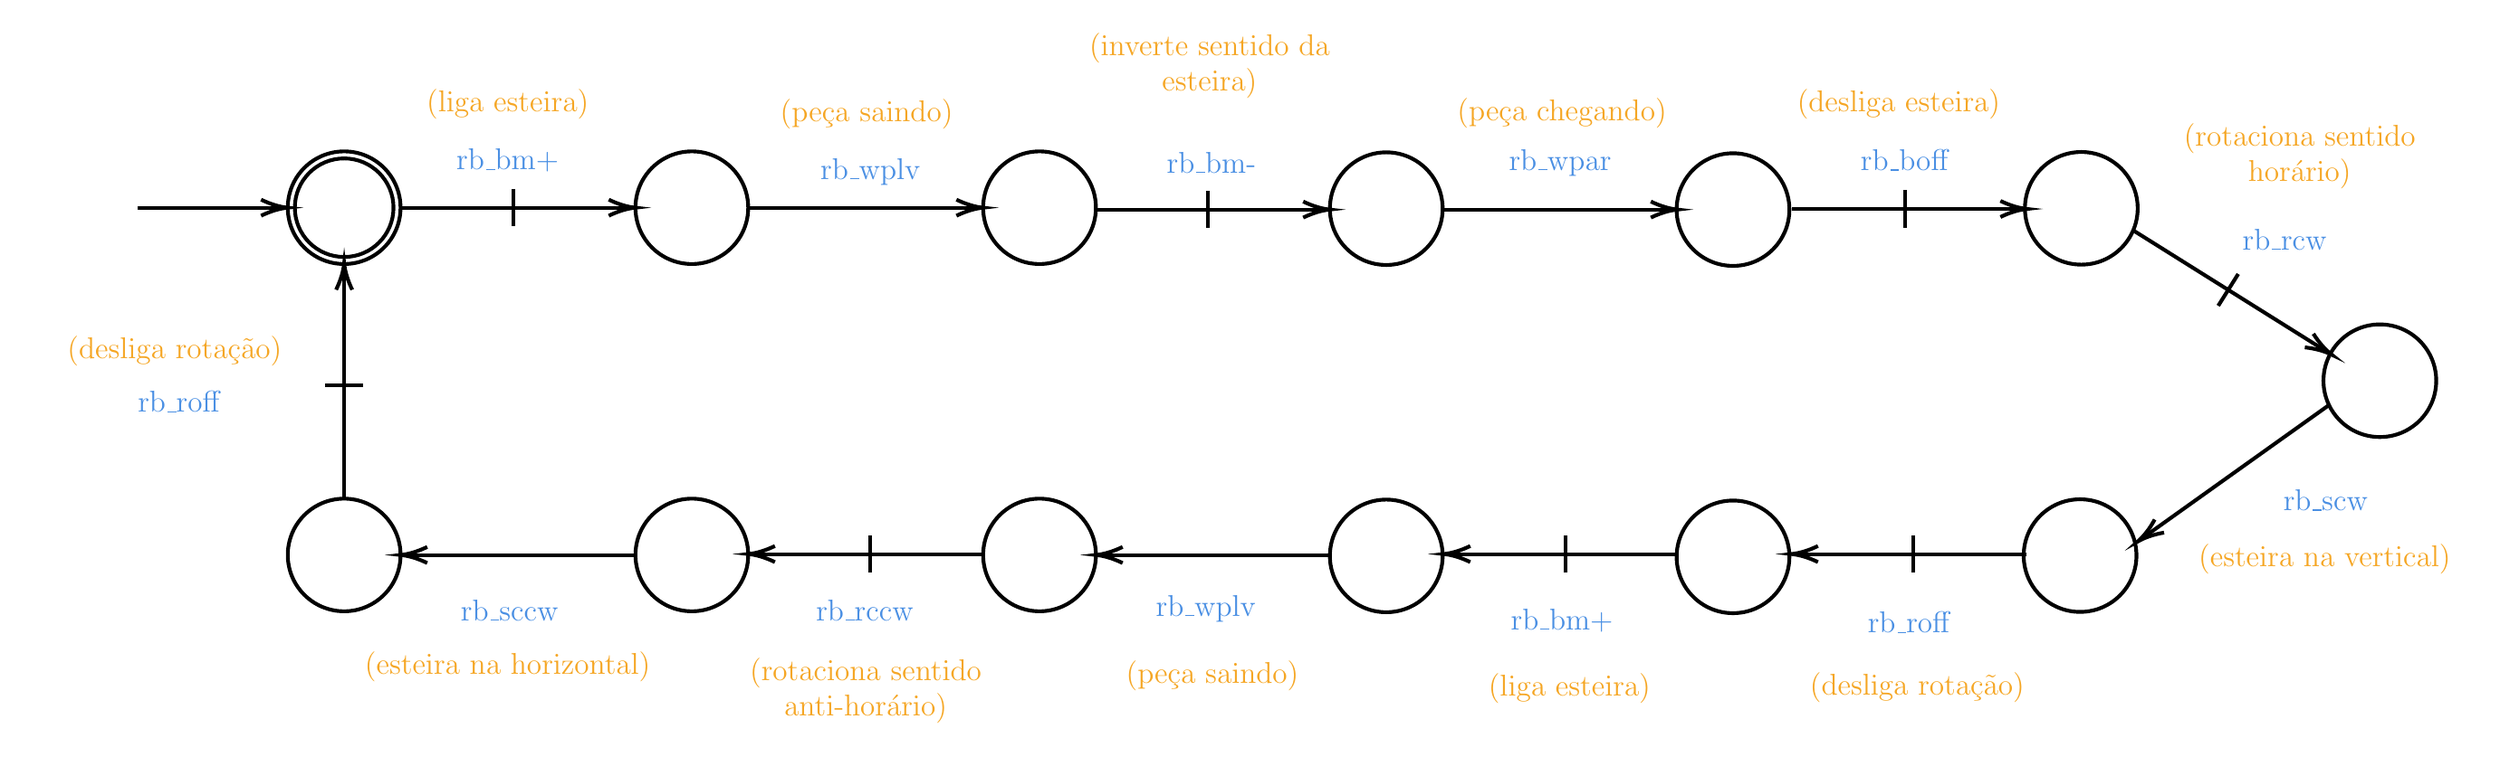
\begin{tikzpicture}[x=0.75pt,y=0.75pt,yscale=-1,xscale=1]
%uncomment if require: \path (0,3420); %set diagram left start at 0, and has height of 3420

%Shape: Circle [id:dp5674605100392998] 
\draw  [line width=1.5]  (195,2385.5) .. controls (195,2368.93) and (208.43,2355.5) .. (225,2355.5) .. controls (241.57,2355.5) and (255,2368.93) .. (255,2385.5) .. controls (255,2402.07) and (241.57,2415.5) .. (225,2415.5) .. controls (208.43,2415.5) and (195,2402.07) .. (195,2385.5) -- cycle ;
%Shape: Circle [id:dp6192867041908257] 
\draw  [line width=1.5]  (198.75,2385.5) .. controls (198.75,2371) and (210.5,2359.25) .. (225,2359.25) .. controls (239.5,2359.25) and (251.25,2371) .. (251.25,2385.5) .. controls (251.25,2400) and (239.5,2411.75) .. (225,2411.75) .. controls (210.5,2411.75) and (198.75,2400) .. (198.75,2385.5) -- cycle ;
%Straight Lines [id:da6462872823460075] 
\draw [line width=1.5]    (115,2385.5) -- (192,2385.5) ;
\draw [shift={(195,2385.5)}, rotate = 180] [color={rgb, 255:red, 0; green, 0; blue, 0 }  ][line width=1.5]    (14.21,-4.28) .. controls (9.04,-1.82) and (4.3,-0.39) .. (0,0) .. controls (4.3,0.39) and (9.04,1.82) .. (14.21,4.28)   ;
%Straight Lines [id:da8581814908068373] 
\draw [line width=1.5]    (255,2385.5) -- (278,2385.5) -- (377,2385.5) ;
\draw [shift={(380,2385.5)}, rotate = 180] [color={rgb, 255:red, 0; green, 0; blue, 0 }  ][line width=1.5]    (14.21,-4.28) .. controls (9.04,-1.82) and (4.3,-0.39) .. (0,0) .. controls (4.3,0.39) and (9.04,1.82) .. (14.21,4.28)   ;
%Straight Lines [id:da25273542205681165] 
\draw [line width=1.5]    (315,2375.5) -- (315,2395.5) ;

%Shape: Circle [id:dp4996334188130662] 
\draw  [line width=1.5]  (380,2385.5) .. controls (380,2368.93) and (393.43,2355.5) .. (410,2355.5) .. controls (426.57,2355.5) and (440,2368.93) .. (440,2385.5) .. controls (440,2402.07) and (426.57,2415.5) .. (410,2415.5) .. controls (393.43,2415.5) and (380,2402.07) .. (380,2385.5) -- cycle ;
%Straight Lines [id:da0776500910074196] 
\draw [line width=1.5]    (440,2385.5) -- (562,2385.5) ;
\draw [shift={(565,2385.5)}, rotate = 180] [color={rgb, 255:red, 0; green, 0; blue, 0 }  ][line width=1.5]    (14.21,-4.28) .. controls (9.04,-1.82) and (4.3,-0.39) .. (0,0) .. controls (4.3,0.39) and (9.04,1.82) .. (14.21,4.28)   ;
%Shape: Circle [id:dp48278690481813924] 
\draw  [line width=1.5]  (565,2385.5) .. controls (565,2368.93) and (578.43,2355.5) .. (595,2355.5) .. controls (611.57,2355.5) and (625,2368.93) .. (625,2385.5) .. controls (625,2402.07) and (611.57,2415.5) .. (595,2415.5) .. controls (578.43,2415.5) and (565,2402.07) .. (565,2385.5) -- cycle ;
%Shape: Circle [id:dp28843785898089935] 
\draw  [line width=1.5]  (934,2386.5) .. controls (934,2369.93) and (947.43,2356.5) .. (964,2356.5) .. controls (980.57,2356.5) and (994,2369.93) .. (994,2386.5) .. controls (994,2403.07) and (980.57,2416.5) .. (964,2416.5) .. controls (947.43,2416.5) and (934,2403.07) .. (934,2386.5) -- cycle ;
%Shape: Circle [id:dp9961852091595447] 
\draw  [line width=1.5]  (934,2571.5) .. controls (934,2554.93) and (947.43,2541.5) .. (964,2541.5) .. controls (980.57,2541.5) and (994,2554.93) .. (994,2571.5) .. controls (994,2588.07) and (980.57,2601.5) .. (964,2601.5) .. controls (947.43,2601.5) and (934,2588.07) .. (934,2571.5) -- cycle ;
%Shape: Circle [id:dp4895093457517301] 
\draw  [line width=1.5]  (565,2570.5) .. controls (565,2553.93) and (578.43,2540.5) .. (595,2540.5) .. controls (611.57,2540.5) and (625,2553.93) .. (625,2570.5) .. controls (625,2587.07) and (611.57,2600.5) .. (595,2600.5) .. controls (578.43,2600.5) and (565,2587.07) .. (565,2570.5) -- cycle ;
%Shape: Circle [id:dp8842647522886835] 
\draw  [line width=1.5]  (380,2570.5) .. controls (380,2553.93) and (393.43,2540.5) .. (410,2540.5) .. controls (426.57,2540.5) and (440,2553.93) .. (440,2570.5) .. controls (440,2587.07) and (426.57,2600.5) .. (410,2600.5) .. controls (393.43,2600.5) and (380,2587.07) .. (380,2570.5) -- cycle ;
%Shape: Circle [id:dp04698640994378667] 
\draw  [line width=1.5]  (195,2570.5) .. controls (195,2553.93) and (208.43,2540.5) .. (225,2540.5) .. controls (241.57,2540.5) and (255,2553.93) .. (255,2570.5) .. controls (255,2587.07) and (241.57,2600.5) .. (225,2600.5) .. controls (208.43,2600.5) and (195,2587.07) .. (195,2570.5) -- cycle ;
%Straight Lines [id:da8880436975826103] 
\draw [line width=1.5]    (565,2570) -- (542,2570) -- (443,2570) ;
\draw [shift={(440,2570)}, rotate = 360] [color={rgb, 255:red, 0; green, 0; blue, 0 }  ][line width=1.5]    (14.21,-4.28) .. controls (9.04,-1.82) and (4.3,-0.39) .. (0,0) .. controls (4.3,0.39) and (9.04,1.82) .. (14.21,4.28)   ;
%Straight Lines [id:da05524259312364732] 
\draw [line width=1.5]    (505,2580) -- (505,2560) ;

%Shape: Circle [id:dp6891516069422883] 
\draw  [line width=1.5]  (749.5,2386) .. controls (749.5,2369.43) and (762.93,2356) .. (779.5,2356) .. controls (796.07,2356) and (809.5,2369.43) .. (809.5,2386) .. controls (809.5,2402.57) and (796.07,2416) .. (779.5,2416) .. controls (762.93,2416) and (749.5,2402.57) .. (749.5,2386) -- cycle ;
%Shape: Circle [id:dp8615598456278082] 
\draw  [line width=1.5]  (749.5,2571) .. controls (749.5,2554.43) and (762.93,2541) .. (779.5,2541) .. controls (796.07,2541) and (809.5,2554.43) .. (809.5,2571) .. controls (809.5,2587.57) and (796.07,2601) .. (779.5,2601) .. controls (762.93,2601) and (749.5,2587.57) .. (749.5,2571) -- cycle ;
%Straight Lines [id:da07720415593040353] 
\draw [line width=1.5]    (624.5,2386.5) -- (647.5,2386.5) -- (746.5,2386.5) ;
\draw [shift={(749.5,2386.5)}, rotate = 180] [color={rgb, 255:red, 0; green, 0; blue, 0 }  ][line width=1.5]    (14.21,-4.28) .. controls (9.04,-1.82) and (4.3,-0.39) .. (0,0) .. controls (4.3,0.39) and (9.04,1.82) .. (14.21,4.28)   ;
%Straight Lines [id:da42064533442896535] 
\draw [line width=1.5]    (684.5,2376.5) -- (684.5,2396.5) ;

%Straight Lines [id:da052365169905879805] 
\draw [line width=1.5]    (809.5,2386.5) -- (832.5,2386.5) -- (931.5,2386.5) ;
\draw [shift={(934.5,2386.5)}, rotate = 180] [color={rgb, 255:red, 0; green, 0; blue, 0 }  ][line width=1.5]    (14.21,-4.28) .. controls (9.04,-1.82) and (4.3,-0.39) .. (0,0) .. controls (4.3,0.39) and (9.04,1.82) .. (14.21,4.28)   ;
%Straight Lines [id:da932484850113712] 
\draw [line width=1.5]    (1176.67,2397.41) -- (1196.15,2409.63) -- (1280.03,2462.23) ;
\draw [shift={(1282.57,2463.82)}, rotate = 212.09] [color={rgb, 255:red, 0; green, 0; blue, 0 }  ][line width=1.5]    (14.21,-4.28) .. controls (9.04,-1.82) and (4.3,-0.39) .. (0,0) .. controls (4.3,0.39) and (9.04,1.82) .. (14.21,4.28)   ;
%Straight Lines [id:da03773841947915524] 
\draw [line width=1.5]    (1232.81,2420.82) -- (1222.19,2437.76) ;

%Shape: Circle [id:dp05559103033681945] 
\draw  [line width=1.5]  (1278.18,2477.67) .. controls (1278.18,2461.1) and (1291.61,2447.67) .. (1308.18,2447.67) .. controls (1324.75,2447.67) and (1338.18,2461.1) .. (1338.18,2477.67) .. controls (1338.18,2494.24) and (1324.75,2507.67) .. (1308.18,2507.67) .. controls (1291.61,2507.67) and (1278.18,2494.24) .. (1278.18,2477.67) -- cycle ;
%Straight Lines [id:da242633953186149] 
\draw [line width=1.5]    (1281.03,2490.71) -- (1262.31,2504.08) -- (1181.75,2561.61) ;
\draw [shift={(1179.31,2563.36)}, rotate = 324.47] [color={rgb, 255:red, 0; green, 0; blue, 0 }  ][line width=1.5]    (14.21,-4.28) .. controls (9.04,-1.82) and (4.3,-0.39) .. (0,0) .. controls (4.3,0.39) and (9.04,1.82) .. (14.21,4.28)   ;
%Shape: Circle [id:dp6253186010208329] 
\draw  [line width=1.5]  (1119.33,2385.83) .. controls (1119.33,2369.26) and (1132.76,2355.83) .. (1149.33,2355.83) .. controls (1165.9,2355.83) and (1179.33,2369.26) .. (1179.33,2385.83) .. controls (1179.33,2402.4) and (1165.9,2415.83) .. (1149.33,2415.83) .. controls (1132.76,2415.83) and (1119.33,2402.4) .. (1119.33,2385.83) -- cycle ;
%Shape: Circle [id:dp8714008127758552] 
\draw  [line width=1.5]  (1118.67,2570.83) .. controls (1118.67,2554.26) and (1132.1,2540.83) .. (1148.67,2540.83) .. controls (1165.24,2540.83) and (1178.67,2554.26) .. (1178.67,2570.83) .. controls (1178.67,2587.4) and (1165.24,2600.83) .. (1148.67,2600.83) .. controls (1132.1,2600.83) and (1118.67,2587.4) .. (1118.67,2570.83) -- cycle ;
%Straight Lines [id:da6634153780153438] 
\draw [line width=1.5]    (995.5,2386.17) -- (1018.5,2386.17) -- (1117.5,2386.17) ;
\draw [shift={(1120.5,2386.17)}, rotate = 180] [color={rgb, 255:red, 0; green, 0; blue, 0 }  ][line width=1.5]    (14.21,-4.28) .. controls (9.04,-1.82) and (4.3,-0.39) .. (0,0) .. controls (4.3,0.39) and (9.04,1.82) .. (14.21,4.28)   ;
%Straight Lines [id:da5974473784438661] 
\draw [line width=1.5]    (1055.5,2376.17) -- (1055.5,2396.17) ;

%Straight Lines [id:da2167698853056801] 
\draw [line width=1.5]    (935,2570) -- (912,2570) -- (813,2570) ;
\draw [shift={(810,2570)}, rotate = 360] [color={rgb, 255:red, 0; green, 0; blue, 0 }  ][line width=1.5]    (14.21,-4.28) .. controls (9.04,-1.82) and (4.3,-0.39) .. (0,0) .. controls (4.3,0.39) and (9.04,1.82) .. (14.21,4.28)   ;
%Straight Lines [id:da0864350441474886] 
\draw [line width=1.5]    (875,2580) -- (875,2560) ;

%Straight Lines [id:da9199456869869072] 
\draw [line width=1.5]    (1120,2570) -- (1097,2570) -- (998,2570) ;
\draw [shift={(995,2570)}, rotate = 360] [color={rgb, 255:red, 0; green, 0; blue, 0 }  ][line width=1.5]    (14.21,-4.28) .. controls (9.04,-1.82) and (4.3,-0.39) .. (0,0) .. controls (4.3,0.39) and (9.04,1.82) .. (14.21,4.28)   ;
%Straight Lines [id:da32780443389976943] 
\draw [line width=1.5]    (1060,2580) -- (1060,2560) ;

%Straight Lines [id:da10233572054292561] 
\draw [line width=1.5]    (628,2570.5) -- (750,2570.5) ;
\draw [shift={(625,2570.5)}, rotate = 0] [color={rgb, 255:red, 0; green, 0; blue, 0 }  ][line width=1.5]    (14.21,-4.28) .. controls (9.04,-1.82) and (4.3,-0.39) .. (0,0) .. controls (4.3,0.39) and (9.04,1.82) .. (14.21,4.28)   ;
%Straight Lines [id:da6708865710001901] 
\draw [line width=1.5]    (258,2570.5) -- (380,2570.5) ;
\draw [shift={(255,2570.5)}, rotate = 0] [color={rgb, 255:red, 0; green, 0; blue, 0 }  ][line width=1.5]    (14.21,-4.28) .. controls (9.04,-1.82) and (4.3,-0.39) .. (0,0) .. controls (4.3,0.39) and (9.04,1.82) .. (14.21,4.28)   ;
%Straight Lines [id:da08343422556470292] 
\draw [line width=1.5]    (225,2540) -- (225,2517) -- (225,2418) ;
\draw [shift={(225,2415)}, rotate = 90] [color={rgb, 255:red, 0; green, 0; blue, 0 }  ][line width=1.5]    (14.21,-4.28) .. controls (9.04,-1.82) and (4.3,-0.39) .. (0,0) .. controls (4.3,0.39) and (9.04,1.82) .. (14.21,4.28)   ;
%Straight Lines [id:da5031168101651777] 
\draw [line width=1.5]    (215,2480) -- (235,2480) ;


% Text Node
\draw (312,2360.5) node  [font=\large] [align=left] {\begin{minipage}[lt]{51.17pt}\setlength\topsep{0pt}
\begin{center}
\textcolor[rgb]{0.29,0.56,0.89}{rb\_bm+}
\end{center}

\end{minipage}};
% Text Node
\draw (312,2330.5) node  [font=\large] [align=left] {\begin{minipage}[lt]{91.55pt}\setlength\topsep{0pt}
\begin{center}
\textcolor[rgb]{0.96,0.65,0.14}{(liga esteira)}
\end{center}

\end{minipage}};
% Text Node
\draw (505,2366.5) node  [font=\large] [align=left] {\begin{minipage}[lt]{68.09pt}\setlength\topsep{0pt}
\begin{center}
\textcolor[rgb]{0.29,0.56,0.89}{rb\_wplv}
\end{center}

\end{minipage}};
% Text Node
\draw (503,2335.5) node  [font=\large] [align=left] {\begin{minipage}[lt]{98.81pt}\setlength\topsep{0pt}
\begin{center}
\textcolor[rgb]{0.96,0.65,0.14}{(peça saindo)}
\end{center}

\end{minipage}};
% Text Node
\draw (872,2361.5) node  [font=\large] [align=left] {\begin{minipage}[lt]{58.23pt}\setlength\topsep{0pt}
\begin{center}
\textcolor[rgb]{0.29,0.56,0.89}{rb\_wpar}
\end{center}

\end{minipage}};
% Text Node
\draw (873,2335) node  [font=\large] [align=left] {\begin{minipage}[lt]{98.81pt}\setlength\topsep{0pt}
\begin{center}
\textcolor[rgb]{0.96,0.65,0.14}{(peça chegando)}
\end{center}

\end{minipage}};
% Text Node
\draw (1279.33,2541.33) node  [font=\large] [align=left] {\begin{minipage}[lt]{57.55pt}\setlength\topsep{0pt}
\begin{center}
\textcolor[rgb]{0.29,0.56,0.89}{rb\_scw}
\end{center}

\end{minipage}};
% Text Node
\draw (1278.83,2572.83) node  [font=\large] [align=left] {\begin{minipage}[lt]{112.65pt}\setlength\topsep{0pt}
\begin{center}
\textcolor[rgb]{0.96,0.65,0.14}{(esteira na vertical)}
\end{center}

\end{minipage}};
% Text Node
\draw (1055.18,2360.17) node  [font=\large] [align=left] {\begin{minipage}[lt]{57.55pt}\setlength\topsep{0pt}
\begin{center}
\textcolor[rgb]{0.29,0.56,0.89}{rb\_boff}
\end{center}

\end{minipage}};
% Text Node
\draw (1052.18,2330.17) node  [font=\large] [align=left] {\begin{minipage}[lt]{112.65pt}\setlength\topsep{0pt}
\begin{center}
\textcolor[rgb]{0.96,0.65,0.14}{(desliga esteira)}
\end{center}

\end{minipage}};
% Text Node
\draw (873,2605.5) node  [font=\large] [align=left] {\begin{minipage}[lt]{57.55pt}\setlength\topsep{0pt}
\begin{center}
\textcolor[rgb]{0.29,0.56,0.89}{rb\_bm+}
\end{center}

\end{minipage}};
% Text Node
\draw (877,2641.5) node  [font=\large] [align=left] {\begin{minipage}[lt]{112.65pt}\setlength\topsep{0pt}
\begin{center}
\textcolor[rgb]{0.96,0.65,0.14}{(liga esteira)}
\end{center}

\end{minipage}};
% Text Node
\draw (683.5,2599) node  [font=\large] [align=left] {\begin{minipage}[lt]{57.55pt}\setlength\topsep{0pt}
\begin{center}
\textcolor[rgb]{0.29,0.56,0.89}{rb\_wplv}
\end{center}

\end{minipage}};
% Text Node
\draw (137,2489) node  [font=\large] [align=left] {\begin{minipage}[lt]{64.47pt}\setlength\topsep{0pt}
\begin{center}
\textcolor[rgb]{0.29,0.56,0.89}{rb\_roff}
\end{center}

\end{minipage}};
% Text Node
\draw (686.5,2361.5) node  [font=\large] [align=left] {\begin{minipage}[lt]{51.17pt}\setlength\topsep{0pt}
\begin{center}
\textcolor[rgb]{0.29,0.56,0.89}{rb\_bm-}
\end{center}

\end{minipage}};
% Text Node
\draw (685.5,2310) node  [font=\large] [align=left] {\begin{minipage}[lt]{108.91pt}\setlength\topsep{0pt}
\begin{center}
\textcolor[rgb]{0.96,0.65,0.14}{(inverte sentido da esteira)}
\end{center}

\end{minipage}};
% Text Node
\draw (1057.5,2606.5) node  [font=\large] [align=left] {\begin{minipage}[lt]{57.55pt}\setlength\topsep{0pt}
\begin{center}
\textcolor[rgb]{0.29,0.56,0.89}{rb\_roff}
\end{center}

\end{minipage}};
% Text Node
\draw (1062,2641) node  [font=\large] [align=left] {\begin{minipage}[lt]{112.65pt}\setlength\topsep{0pt}
\begin{center}
\textcolor[rgb]{0.96,0.65,0.14}{(desliga rotação)}
\end{center}

\end{minipage}};
% Text Node
\draw (687,2635) node  [font=\large] [align=left] {\begin{minipage}[lt]{91.55pt}\setlength\topsep{0pt}
\begin{center}
\textcolor[rgb]{0.96,0.65,0.14}{(peça saindo)}
\end{center}

\end{minipage}};
% Text Node
\draw (1257.51,2402.5) node  [font=\large] [align=left] {\begin{minipage}[lt]{57.55pt}\setlength\topsep{0pt}
\begin{center}
\textcolor[rgb]{0.29,0.56,0.89}{rb\_rcw}
\end{center}

\end{minipage}};
% Text Node
\draw (1265.51,2358.17) node  [font=\large] [align=left] {\begin{minipage}[lt]{112.65pt}\setlength\topsep{0pt}
\begin{center}
\textcolor[rgb]{0.96,0.65,0.14}{(rotaciona sentido horário)}
\end{center}

\end{minipage}};
% Text Node
\draw (502,2600) node  [font=\large] [align=left] {\begin{minipage}[lt]{57.55pt}\setlength\topsep{0pt}
\begin{center}
\textcolor[rgb]{0.29,0.56,0.89}{rb\_rccw}
\end{center}

\end{minipage}};
% Text Node
\draw (502.5,2643) node  [font=\large] [align=left] {\begin{minipage}[lt]{112.65pt}\setlength\topsep{0pt}
\begin{center}
\textcolor[rgb]{0.96,0.65,0.14}{(rotaciona sentido anti-horário)}
\end{center}

\end{minipage}};
% Text Node
\draw (313,2600) node  [font=\large] [align=left] {\begin{minipage}[lt]{57.55pt}\setlength\topsep{0pt}
\begin{center}
\textcolor[rgb]{0.29,0.56,0.89}{rb\_sccw}
\end{center}

\end{minipage}};
% Text Node
\draw (312,2630) node  [font=\large] [align=left] {\begin{minipage}[lt]{126.02pt}\setlength\topsep{0pt}
\begin{center}
\textcolor[rgb]{0.96,0.65,0.14}{(esteira na horizontal)}
\end{center}

\end{minipage}};
% Text Node
\draw (134.75,2462) node  [font=\large] [align=left] {\begin{minipage}[lt]{112.65pt}\setlength\topsep{0pt}
\begin{center}
\textcolor[rgb]{0.96,0.65,0.14}{(desliga rotação)}
\end{center}

\end{minipage}};


\end{tikzpicture}}
        \caption{\textit{Rotary table} completo.}
        \label{fig:sistema}
    \end{figure}
\end{frame}




